\documentclass[10pt, letterpaper]{article}

% Inhaltsverzeichnis für Pakettypen (nur für Übersicht im Header, wird nicht im Dokument angezeigt)
% 1. Seitenlayout und Ränder
% 2. Sprache und Zeichensatz
% 3. Mathematik und Theorem-Umgebungen
% 4. Eigene Makros
% 5. Diagramme und Grafiken
% 6. Tabellen und Aufzählungen
% 7. Inhaltsverzeichnis
% 8. Abschnittsüberschriften
% 9. Abstrakt-Umgebung
% 10. Todos/Notizen
% 11. Rahmen/Box-Umgebungen
% 12. Python-Integration
% 13. Literaturverwaltung
% 14. Hyperlinks
% 15. Absatzeinstellungen
% 16. Umgebungen
% 17  Graphik
% 00. Titel und Autor

% --- 1. Seitenlayout und Ränder ---
\usepackage[margin=3cm]{geometry}

% --- 2. Sprache und Zeichensatz ---
\usepackage[english]{babel}
\usepackage[T1]{fontenc}
\usepackage[utf8]{inputenc}

% --- 3. Mathematik und Theorem-Umgebungen ---
\usepackage{amsmath, amssymb, amsthm}
\usepackage{mathrsfs}
\DeclareMathOperator{\WF}{WF}

% --- 4. Eigene Makros ---
\usepackage{xcolor}
\newcommand{\SKP}{\langle\cdot,\cdot\rangle}
\newcommand{\R}{\mathbb{R}}
\newcommand{\N}{\mathbb{N}}
\newcommand{\Q}{\mathbb{Q}}
\newcommand{\Z}{\mathbb{Z}}
\newcommand{\C}{\mathbb{C}}
\newcommand{\entwurf}[1]{\textcolor{red}{#1}}

% --- 5. Diagramme und Grafiken ---
\usepackage{graphicx}
\usepackage{tikz}
\usetikzlibrary{decorations.pathreplacing, arrows.meta, positioning}
\usepackage{tikz-cd}

% --- 6. Tabellen und Aufzählungen ---
\usepackage{enumitem}
\setlist[itemize]{left=0.5cm}

\newenvironment{romanenum}[1][]
  {%
    \ifx&#1&
    \else
      \textbf{#1}\quad
    \fi
    \begin{enumerate}[label=\roman*)]
  }
  {%
    \end{enumerate}%
  }

% --- 7. Inhaltsverzeichnis ---
\usepackage{tocloft}
\renewcommand{\cftsecfont}{\footnotesize}
\renewcommand{\cftsubsecfont}{\footnotesize}
\renewcommand{\cftsubsubsecfont}{\footnotesize}
\renewcommand{\cftsecpagefont}{\footnotesize}
\renewcommand{\cftsubsecpagefont}{\footnotesize}
\renewcommand{\cftsubsubsecpagefont}{\footnotesize}
\usepackage{etoc}

% --- 8. Abschnittsüberschriften ---
\usepackage{titlesec}
\titleformat{\section}{\normalfont\large\bfseries}{\thesection}{1em}{}
\titleformat{\subsection}{\normalfont\normalsize\bfseries}{\thesubsection}{0.5em}{}
\titleformat{\subsubsection}{\normalfont\normalsize\bfseries}{\thesubsubsection}{0.5em}{}
\setcounter{secnumdepth}{4}

% --- 9. Abstrakt-Umgebung ---
\usepackage{changepage}
\renewenvironment{abstract}
  {
    \begin{adjustwidth}{1.5cm}{1.5cm}
    \small
    \textsc{Abstract. –}%
  }
  {
    \end{adjustwidth}
  }

% --- 10. Todos/Notizen ---
\usepackage{todonotes}

% --- 11. Rahmen/Box-Umgebungen ---
\usepackage{mdframed}
\usepackage{tcolorbox}
\colorlet{shadecolor}{gray!25}

\newenvironment{customTheorem}
  {\vspace{10pt}%
   \begin{mdframed}[
     backgroundcolor=gray!20,
     linewidth=0pt,
     innertopmargin=10pt,
     innerbottommargin=10pt,
     skipabove=\dimexpr\topsep+\ht\strutbox\relax,
     skipbelow=\topsep,
   ]}
  {\end{mdframed}
   \vspace{10pt}%
  }

% --- 12. Python-Integration ---
% (Deaktiviert in dieser Version, aktiviere bei Bedarf)
% \usepackage{pythontex}
% \usepackage[makestderr]{pythontex}

% --- 13. Literaturverwaltung ---
\usepackage{csquotes}
\usepackage[backend=biber, style=alphabetic, citestyle=alphabetic]{biblatex}
\addbibresource{bibliography.bib}

% --- 14. Hyperlinks ---
\usepackage{hyperref}
\hypersetup{
  colorlinks   = true,
  urlcolor     = blue,
  linkcolor    = blue,
  citecolor    = blue,
  frenchlinks  = true
}

% --- 15. Absatzeinstellungen ---
\usepackage[parfill]{parskip}
\sloppy

% --- 16. Umgebungen ---
\usepackage{thmtools}

\newcommand{\CustomHeading}[3]{%
  \par\medskip\noindent%
  \textbf{#1 #2} \textnormal{(#3)}.\enskip%
}

\newenvironment{DEF}[2]{\begin{unitbox}\CustomHeading{Definition}{#1}{#2}}{\end{unitbox}}
\newenvironment{PROP}[2]{\begin{unitbox}\CustomHeading{Proposition}{#1}{#2}}{\end{unitbox}}
\newenvironment{THEO}[2]{\begin{unitbox}\CustomHeading{Theorem}{#1}{#2}}{\end{unitbox}}
\newenvironment{LEM}[2]{\begin{unitbox}\CustomHeading{Lemma}{#1}{#2}}{\end{unitbox}}
\newenvironment{KORO}[2]{\begin{unitbox}\CustomHeading{Corollar}{#1}{#2}}{\end{unitbox}}
\newenvironment{REM}[2]{\begin{unitbox}\CustomHeading{Remark}{#1}{#2}}{\end{unitbox}}
\newenvironment{EXA}[2]{\begin{unitbox}\CustomHeading{Example}{#1}{#2}}{\end{unitbox}}
\newenvironment{STUD}[2]{\begin{unitbox}\CustomHeading{Study}{#1}{#2}}{\end{unitbox}}
\newenvironment{CONC}[2]{\begin{unitbox}\CustomHeading{Concept}{#1}{#2}}{\end{unitbox}}

\newenvironment{PROOF}
  {\begin{proof}}%
{\end{proof}}

% --- Unit Umgebung für Source-Inhalte ---
\usepackage{mdframed}
\newmdenv[
  linewidth=1pt,
  topline=false,
  bottomline=false,
  rightline=false,
  leftmargin=0cm,
  rightmargin=0cm,
  skipabove=10pt,
  skipbelow=10pt,
  innertopmargin=0.5\baselineskip,
  innerbottommargin=0.5\baselineskip,
  backgroundcolor=gray!10,
  linecolor=gray
]{unitbox}

\newenvironment{unit}[1]
  {\begin{unitbox}\textbf{Unit #1}\par\smallskip}
  {\end{unitbox}}

% --- 17. Graphik ---
\usepackage{graphicx}
\graphicspath{ {./images/} }
\usepackage[export]{adjustbox}

% --- 00. Titel und Autor ---
\title{Mein Titel}
\author{Tim Jaschik}
\date{\today}

\begin{document}

\maketitle
\rule{\textwidth}{0.5pt}
\begin{abstract}
Kurze Beschreibung …
\end{abstract}
\rule{\textwidth}{0.5pt}
\vspace{0.5cm}

\tableofcontents

\pagebreak




\section{Liegruppen}


\subsection*{1.1 Definition}
Eine Liegruppe ( $G, \cdot$ ) ist eine differenzierbare Mannigfaltigkeit zusammen mit einer Gruppenstruktur, sodass die Abbildung

$$
G \times G \rightarrow G, \quad(g, h) \mapsto g h^{-1}
$$

differenzierbar ist.

\subsection*{1.2 Beispiele}
a) Ist $G$ eine endliche Gruppe, so ist $G$ eine 0-dimensionale Liegruppe.\\
b) $\mathbb{R}^{n}, \mathbb{C}^{n}$ sind abelsche Liegruppen. Ebenso ist $S^{1}$ eine abelsche Liegruppe.\\
c) $G L(n, k)$ ist für $k=\mathbb{R}$ oder $k=\mathbb{C}$ eine Liegruppe.\\
d) Die bekannten Matrizengruppen, z.B. $O(n), S L(n, \mathbb{R}), U(n), S O(n)$ sind Liegruppen, wie man leicht mit dem Satz vom regulären Wert beweist (Übungsaufgabe!).\\
e) Sind $G$ und $H$ Liegruppen, so ist $G \times H$ eine Liegruppe. Insbesondere ist $T^{2}=S^{1} \times S^{1}$ eine Liegruppe.\\
f) Die affine Gruppe

$$
\operatorname{Aff}_{n}(k)=\left(G L(n, k) \times k^{n},((A, v),(B, w)) \mapsto(A B, A w+b)\right)
$$

ist eine Liegruppe. Aff ${ }_{1}(k)$ ist die einzige zusammenhängende zweidimensionale nicht abelsche Liegruppe.

\subsection*{1.3 Definition}
Sei $G$ eine Liegruppe und $H \subseteq G$ eine Untergruppe, so heißt $H$ eine Unterliegruppe, falls $H$ eine Untermannigfaltigkeit ist.

\subsection*{1.4 Beispiele}
a) $O(n) \subseteq G L(n, \mathbb{R})$ ist eine Unterliegruppe.\\
b) $M_{\alpha}:=\left\{\left(e^{i t}, e^{i t \alpha}\right) \mid t \in \mathbb{R}\right\} \subseteq T^{2}$ ist eine Untergruppe für $\alpha \in \mathbb{R}$. Für $\alpha \in \mathbb{Q}$ ist $M_{\alpha}$ eine Unterliegruppe, für $\alpha \in \mathbb{R} \backslash \mathbb{Q}$ nicht. (Übungsaufgabe!)\\
c) $N_{n}(k)=\left\{\left(a_{i j}\right) \in G L(n, k) \mid a_{i j}=0\right.$ für $\left.i>j, a_{i i}=1, i=1, \ldots, n\right\}$ ist eine Untergruppe.

\subsection*{1.5 Satz}
Ist $H \subseteq G$ eine Unterliegruppe, so ist $H \subseteq G$ abgeschlossen.

Beweis: Angenommen, es existiert ein $g \in \bar{H} \backslash H$. Sei ( $U, F$ ) eine Untermannigfaltigkeitskarte von $H$ um 1. Dann ist $g U^{-1}=\left\{x \in G \mid x^{-1} g \in U\right\} \subseteq G$ eine offene Umgebung von $g$, also $g U^{-1} \cap H \neq \emptyset$.\\
Sei $h \in g U^{-1} \cap H$, dann ist $h^{-1} g \notin H$, da $g \notin H$. Wegen $g^{-1} h \in U^{-1}$ ist also $h^{-1} g \in U \backslash H$. Also existiert eine offene Umgebung $V \subseteq U$ von $h^{-1} g \in V$ mit $V \cap H=\emptyset$, also ist $h V$ eine offene Umgebung von $g$ mit $h V \cap H=(h(V \cap H))=$ $\emptyset$. Widerspruch!

\subsection*{1.6 Satz}
Jede abgeschlossen Untergruppe einer Liegruppe ist eine Unterliegruppe.\\
Der Beweis wird später gegeben.

\subsection*{1.7 Definiton}
Ein Homomorphismus (bzw. ein Isomorphismus) $f: G \rightarrow H$ zwischen Liegruppen heißt ein Liegruppenhomomorphismus (bzw. -isomorphismus), falls er zusätzlich differenzierbar ist.

\subsection*{1.8 Beispiele}
Die Abbildungen\\
a) $S^{1} \rightarrow S O(2), e^{i t} \rightarrow\binom{\cos t-\sin t}{\sin t \cos t}$\\
b) $S^{1} \rightarrow T^{2}, t \mapsto\left(e^{i t}, e^{i t \alpha}\right), \alpha \in \mathbb{Q}$\\
c) $\mathbb{R} \rightarrow S^{1}, t \rightarrow e^{i t}$\\
d) det : $G l(n, \mathbb{R}) \rightarrow \mathbb{R}^{\star}$\\
e) konj : $G \rightarrow G, x \mapsto g x g^{-1}$\\
sind Liegruppenhomomorphismen.\\
Die Abbildungen\\
f) $\mathbb{R} \rightarrow N_{1}(\mathbb{R}), x \mapsto\left(\begin{array}{ll}1 & x \\ 0 & 1\end{array}\right)$\\
g) $\mathbb{R} \rightarrow \mathcal{L}_{+}^{\uparrow}(1), x \mapsto\left(\begin{array}{cc}\cos h x & \sin h x \\ \sin h x & \cos h x\end{array}\right)$\\
h) $\operatorname{Aff}(k) \rightarrow\left\{\left.\left(\begin{array}{cc}A & b \\ 0 & 1\end{array}\right) \right\rvert\, A \in G L(n, k), b \in \mathbb{R}^{n}\right\}(X, v) \mapsto\left(\begin{array}{cc}X & v \\ 0 & 1\end{array}\right)$ sind Liegruppenisomorphismen.

\subsection*{1.9 Definition}
Sei $G$ eine Liegruppe, $M$ eine Mannigfaltigkeit. Eine differenzierbare Abbildung $\phi: G \times M \rightarrow M$ heißt eine $G-$ (Links)Aktion, falls gilt\\
(1) $\phi\left(g_{1} g_{2}, x\right)=\phi\left(g_{1}, \phi\left(g_{2}, x\right)\right)$.\\
(2) $\phi(1, x)=x$ für alle $x \in M$.

Statt $\phi(g, x)$ schreibt man meist $g x$. Analog sind Rechtsaktionen definiert. Man schreibt statt $\phi(g, \cdot)=L_{g}$ für Linksaktionen bzw. $\phi(\cdot, g)=R_{g}$ für Rechtsaktionen. Eine Mannigfaltigkeit zusammen mit einer $G$-Aktion heißt $G$-Mannigfaltigkeit.

\subsection*{1.10 Bemerkung}
Offenbar ist jede Liegruppe selbst eine $G$-Mannigfaltigkeit.

\subsection*{1.11 Beispiele}
a) Sei $G=S O(n)$ und $M=S^{m}$ mit $n \leq m+1$.

$$
\phi: G \times M \rightarrow M,(A, v) \mapsto\binom{A}{I} v
$$

ist eine $G$-Aktion.\\
b) Sei $G=\operatorname{Aff}(k) \times k^{n}, M=k^{n}$.

$$
\phi: G \times k^{n} \rightarrow k^{n},((A, v), x) \mapsto A x+v
$$

ist eine G-Aktion, denn

$$
\begin{aligned}
& \phi((A, v) \cdot(B, w), x)=A B x+A w+v \text { und } \\
& \phi((A, v), \phi((B, w), x))=\phi((A, v), B x+w)=A B x+A w+v
\end{aligned}
$$

\subsection*{1.12 Übungsaufgaben}
a) Jede offene Untergruppe einer Liegruppe ist auch abgeschlossen.\\
b) Ist $G$ zusammenhängend, $V \subseteq G$ offen mit $1 \in V$, so gilt $\bigcup_{i=1}^{\infty} V^{i}=G$.\\
c) Sei $G$ Liegruppe, $G_{0} \subseteq G$ die Zusammenhangskomponente der 1. Dann ist $G_{0}$ ein Normalteiler.\\
d) Zeigen Sie: $S O(n), S U(n)$ und $S O^{\uparrow}(1, n-1)$ sind zusammenhängende Liegruppen. Was folgt daraus für $O(n)$ und $O(1, n-1)$ ?\\
e) Zeigen Sie: $S^{1} \times S U(n) \rightarrow U(n)$ ist eine $n$-fache Überlagerung.\\
f) Zeigen Sie:

$$
\begin{aligned}
G L(n, \mathbb{R}) & \cong O(n) \times \mathbb{R}^{\frac{1}{2} n(n+1)} \\
G L(n, \mathbb{C}) & \cong U(n) \times \mathbb{R}^{n^{2}}
\end{aligned}
$$


\pagebreak

\section{Invariante Vektorfelder und Differenzialformen}
\subsection*{2.1 Definition}
Sei $M$ eine $G$-Mannigfaltigkeit. Ein Vektorfeld $v \in \Gamma T M=: \mathcal{V}(M)$ heißt linksinvariant, falls gilt

$$
\left.d L_{g}\right|_{x}(v(x))=v(g x)
$$

für alle $g \in G, x \in M$. Den Raum der linksinvarianten Vektorfelder auf $M$ bezeichnen wir mit $\mathcal{V}_{G}(M)$.

\subsection*{2.2 Erinnerung}
Durch $[\cdot, \cdot]: \mathcal{V}(M) \rightarrow \mathcal{V} M$ ist eine bilineare, schiefsymmetrische Abbildung gegeben durch $[v, w] f=v(w f)-w(f)$ für alle $f \in C^{\infty}(M)$. Ist $f: M \rightarrow \widetilde{M}$ eine differenzierbare Abbildung und $\operatorname{sind} v, w \in \mathcal{V}(M)$ und $\tilde{v}, \tilde{w} \in \mathcal{V}(\widetilde{M})$ mit

$$
d f_{x}(v(x))=\tilde{v}(f(x))
$$

und

$$
d f_{x}(w(x))=\tilde{w}(f(x))
$$

für alle $x \in M$ (kurz: $f_{\star} v=\tilde{v}$ und $f_{\star} w=\tilde{w}$ ), so gilt: $f_{\star}([v, w])=[\tilde{v}, \tilde{w}]$. Eine weitere Möglichkeit, die [, ] zu definieren, ist wie folgt gegeben:

\subsection*{2.3 Definition und Satz}
Sind $X, Y$ Vektorfelder auf einer Mannigfaltigkeit und sei $\phi^{(X)}$ der maximale lokale Fluss zu $X$,

$$
\begin{aligned}
& \phi_{t}^{(X)}:=\phi^{(X)}(t, \cdot) \\
& \left(\phi_{t}^{(X)}\right)_{*}(Y)(p)=\left.d \phi_{t}^{(X)}\right|_{\phi_{t}^{-1}(p)}(Y)
\end{aligned}
$$

dann ist die Lieableitung von $Y$ nach $X$ durch

$$
\begin{aligned}
\left(L_{X} Y\right)(p) & =-\left.\frac{d}{d t}\right|_{t=0}\left(\phi_{t}^{(X)}\right)_{*}(Y)(p) \\
& =\lim _{t \rightarrow 0}\left(\frac{1}{t}\left(Y-\left(\phi_{t}\right)_{*} Y\right)(p)\right)
\end{aligned}
$$

definiert. Es gilt $L_{X} Y=[X, Y]$.

\section*{Beweis:}
Vorbemerkung:\\
a) Für $f \in C^{\infty}(M), g: M \rightarrow M$ eine differenzierbare Abbildung, $x \in M, y=g(x)$ gilt

$$
\begin{aligned}
\left(g_{*}\right)(Y)(p)(f) & =d f_{p}\left(\left.d g\right|_{x}(Y)\right. \\
& =d(f \circ g)_{x}(Y)=Y(f \circ g)(x)
\end{aligned}
$$

Also ist für $\phi=\phi^{(X)}$

$$
\left(\phi_{t}\right)_{*}(Y)(p)(f)=Y\left(f \circ \phi_{t}\right)\left(\phi_{-t}(p)\right)
$$

b) Für $h \in C^{\infty}(\mathbb{R})$ mit $h(0)=0$ ist

$$
h(t)=\int_{0}^{1} \frac{\partial}{\partial s} h(t s) d s=t \int_{0}^{1} h^{\prime}(t s) d s=: t \tilde{h}(t)
$$

mit $\tilde{h}(0)=h^{\prime}(0)$. Also ist für $f \in C^{\infty}(M)$

$$
\left(f \circ \phi_{t}-f\right)(q)=t \tilde{f}(q, t)
$$

für $\tilde{f}$ mit $\tilde{f}(q, 0)=\left.d f\right|_{q}(x)=x(f)(q)$. Damit folgt

$$
\begin{aligned}
\left(\phi_{t}\right)_{*}(Y)(p)(f) & =Y\left(f \circ \phi_{t}\right)\left(\phi_{-t}(p)\right) \\
& =Y\left(f\left(\phi_{-t}(p)\right)+t \tilde{f}\left(\phi_{-t}(p), t\right)\right)
\end{aligned}
$$

Also ist

$$
\begin{aligned}
\left.\frac{d}{d t}\right|_{t=0}\left(\phi_{t}\right)_{*}(Y)(p)(f) & =-X Y(f)+Y(\tilde{f}(p, 0)) \\
& =(-X Y(f)+Y X(f))(p)
\end{aligned}
$$

\subsection*{2.4 Definition}
Eine Lie-Algebra ist ein $\mathbb{K}$-Vektorraum $\mathfrak{a}$, versehen mit einer Abbildung

$$
[,]:\left(v_{1}, v_{2}\right) \in \mathfrak{a} \times \mathfrak{a} \mapsto\left[v_{1}, v_{2}\right] \in \mathfrak{a},
$$

welche die folgenden Eigenschaften hat:\\
a) Für alle $v_{1}, v_{2} \in \mathfrak{a}$ ist $\left[v_{1}, v_{2}\right]=-\left[v_{2}, v_{1}\right]$.\\
b) Für alle $v_{1}, v_{2}, v_{3} \in \mathfrak{a}$ und alle $\lambda_{1}, \lambda_{2} \in \mathbb{K}$ ist $\left[\lambda_{1}, v_{1}+\lambda_{2} v_{2}, v_{3}\right]=\lambda_{1}\left[v_{1}, v_{3}\right]+\lambda_{2}\left[v_{2}, v_{3}\right]$.\\
c) Jacobi-Identität: Für alle $v_{1}, v_{2}, v_{3} \in \mathfrak{a}$ ist $\left[\left[v_{1}, v_{2}\right], v_{3}\right]+\left[\left[v_{2}, v_{3}\right], v_{1}\right]+\left[\left[v_{3}, v_{1}\right], v_{2}\right]=0$.

\subsection*{2.5 Beispiele}
a) Der $\mathbb{R}^{3}$ ist zusammen mit $\left[v_{1}, v_{2}\right]:=v_{1} \times v_{2}$, wobei $v_{1} \times v_{2}$ das Vektorprodukt von $v_{1}$ und $v_{2}$ bezeichnet, eine Lie-Algebra.\\
b) Der Vektorraum der $n \times n$-Matrize $M(n, \mathbb{K})$ mit $[A, B]:=A B-B A$ ist eine Lie-Algebra.\\
c) $(\mathcal{V}(M),[\cdot, \cdot])$ ist eine Liealgebra.\\
d) Der Vektorraum der strikten oberen Dreiecksmatrizen

$$
N(n, k)=\left\{\left(a_{i j}\right) \in M(n \times n, k) \mid a_{i j}=0 \text { für } i \geq j\right\}
$$

$N(3, k)$ heißt Heisenberg-Algebra.\\
e) Die Oszillatoralgebra ist definiert als der Vektorraum $N(3, k) \times \mathbb{R}$ mit der Lieklammer definiert durch die Lieklammer auf $N(3, k)$ und

$$
[X, T]=-Y \quad[Y, T]=X \quad[Z, T]=0 .
$$

Für

$$
X=\left(\begin{array}{lll}
0 & 1 & 0 \\
0 & 0 & 0 \\
0 & 0 & 0
\end{array}\right), \quad Y=\left(\begin{array}{lll}
0 & 0 & 0 \\
0 & 0 & 1 \\
0 & 0 & 0
\end{array}\right), \quad Z=\left(\begin{array}{lll}
0 & 0 & 1 \\
0 & 0 & 0 \\
0 & 0 & 0
\end{array}\right)
$$

und das erzeugende $T$ von $\mathbb{R}$.

\subsection*{2.6 Satz}
Sei $M$ eine $G$-Mannigfaltigkeit. Dann ist $\left(\mathcal{V}_{G}(M),[\cdot, \cdot]\right)$ eine Lie-Algebra, d.h. $[\cdot, \cdot]: \mathcal{V}_{G}(M) \times \mathcal{V}_{G}(M) \rightarrow \mathcal{V}_{G}(M)$ ist bilinear und schiefsymmetrisch und erfüllt die Jacobi-Identität $[u[v, w]]+$ zykl. Perm. $=0$.

Beweis: Seien $v, w \in \mathcal{V}_{G}(M)$. Zu zeigen ist nur, dass gilt: $[v, w] \in \mathcal{V}_{G}(M)$. Da $L_{g}$ ein Diffeomorphismus ist, folgt dies aus

$$
\left.d L_{g}\right|_{g^{\prime}}[v, w]\left(g^{\prime}\right)=\left[d L_{g} v, d L_{g} w\right]\left(g g^{\prime}\right)=[v, w]\left(g g^{\prime}\right) .
$$

\subsection*{2.7 Definition}
Sei $M$ eine $G$-Mannigfaltigkeit. Eine Differenzialform $\omega \in \Omega M$ heißt $G$-invariant, falls $L_{g}^{*} \omega=\omega$ gilt für alle $g \in G$. Den Raum der linksinvarianten Formen bezeichnen wir mit $\Omega_{G}(M)$.

\subsection*{2.8 Bemerkungen}
a) Ist $\omega \in \Omega_{G}^{k} M, v \in \mathcal{V}_{G}(M)$, so ist $i_{v} \omega \in \Omega_{G}^{k-1}(M)$.\\
b) Ist $\omega \in \Omega_{G} M$, so ist $d \omega \in \Omega_{G} M$, denn $L_{g}^{*} d \omega=d L_{g}^{*} \omega=d \omega$.\\
c) Sind $\omega, \eta \in \Omega_{G} M$, so ist auch $\omega \wedge \eta \in \Omega_{G} M$.


\pagebreak

\section{Lie-Algebren}

Da jede Lie-Gruppe $G$ eine $G$-Mannigfaltigkeit ist, können wir jetzt auf $G$ auch links-(und rechts-)invariante Vektorfelder und Differenzialformen betrachten.

\subsection*{3.1 Satz}
Die Abbildung

$$
T_{1} G \rightarrow \mathcal{V}_{G}(G), \xi \mapsto\left(\left.g \mapsto d L_{g}\right|_{1}(\xi)\right)=: \xi^{G}
$$

ist ein Isomorphismu von Vektorräumen.\\
Beweis: Offenbar ist die Abbildung linear und ein Inverses ist durch $\mathcal{V}_{G}(G) \rightarrow$ $T_{1} G, v \mapsto v(1)$ gegeben. Zu zeigen ist nur, dass $\xi^{G}$ tatsächlich ein linksinvariantes Vektorfeld definiert:

$$
\left.d L_{g^{\prime}}\right|_{g} \xi^{G}(g)=\left.\left.d L_{g^{\prime}}\right|_{g} \circ d L_{g}\right|_{1}(\xi)=\left.d L_{g^{\prime} g}\right|_{1}(\xi)=\xi^{G}\left(g^{\prime} g\right)
$$

\subsection*{3.2 Beispiele}
a) Da $G L(n, \mathbb{R}) \subseteq M(n \times n, \mathbb{R})$ eine offene Teilmenge ist, ist

$$
T_{1} G L(n, \mathbb{R})=M(n \times n, \mathbb{R})=\mathbb{R}^{n^{2}}=: g \ell(n, \mathbb{R})
$$

Ist $X \in M(n \times n, \mathbb{R})$, so wird $X \in T_{1} G$ durch $e^{t X}$ repräsentiert, also ist

$$
d L_{g}(X)=\left.\frac{d}{d t}\right|_{t=0} g e^{t X}=g X,
$$

also ist $X^{G}(g)=g X$.\\
b) Ist $G \subseteq G L(n, \mathbb{R})$ eine Unterliegruppe, so ist $T_{1} G \subseteq M(n \times n, \mathbb{R})$ ein Untervektorraum und wie in a) ist kanonisch $X^{G}(g)=g X$.\\
c) Mit dem Satz vom regulären Wert zeigt man leicht

$$
\begin{aligned}
& T_{1} O(n)=T_{1} S O(n)=: \operatorname{so}(n)=\left\{X \in g \ell(n, \mathbb{R}) \mid X^{T}=-X\right\} \\
& T_{1} S L(n, \mathbb{R})=\operatorname{sl}(n, \mathbb{R})=\{X \in g \ell(n, \mathbb{R}) \mid \operatorname{tr} X=0\} \\
& T_{1} U(n)=u(n)=\left\{X \in g \ell\left(n, \mathbb{C} \mid \bar{X}^{T}=-X\right\}\right. \\
& T_{1} S U(n)=\operatorname{su}(n)=\{X \in u(n) \mid \operatorname{tr} X=0\}
\end{aligned}
$$

\subsection*{3.3 Korollar}
Jede Liegruppe ist parallelisierbar, d.h. $T G=G \times T_{1} G$. Der Vektorraumbündelisomorphismus ist durch

$$
G \times T_{1} G \rightarrow T G,\left.(g, \xi) \mapsto d L_{g}\right|_{1}(\xi)
$$

gegeben. Damit ist jede Liegruppe orientierbar.

\subsection*{3.4 Satz und Definition}
Auf $T_{1} G=\mathfrak{g}$ ist durch

$$
\mathfrak{g} \times \mathfrak{g} \rightarrow \mathfrak{g},(\xi, \eta) \mapsto\left[\xi^{G}, \eta^{G}\right](1)=:[\xi, \eta]
$$

eine Lieklammer wohldefiniert. ( $\mathfrak{g},[\cdot, \cdot]$ ) heißt die Liealgebra zu $G$.

\subsection*{3.5 Beispiel}
Sind $X, Y \in g \ell(n, \mathbb{R})$, so ist

$$
\begin{aligned}
X^{G}\left(Y^{G}\right)(1) & =\left.\frac{d}{d t}\right|_{t=0} Y^{G}\left(e^{t X}\right) \\
& =\left.\frac{d}{d t}\right|_{t=0}\left(e^{t X} Y\right)=X \cdot Y
\end{aligned}
$$

also

$$
[X, Y]=\left[X^{G}, Y^{G}\right](1)=X \cdot Y-Y \cdot X .
$$

\subsection*{3.6 Definition}
Ist $\mathfrak{g}$ eine Liealgebra, $\mathfrak{h} \subseteq \mathfrak{g}$ ein Untervektorraum, so heißt $\mathfrak{h}$ eine UnterLiealgebra, falls für $\xi, \eta \in \mathfrak{h}$ auch $[\xi, \eta] \in \mathfrak{h}$ gilt.

\subsection*{3.7 Bemerkungen}
a) Ist $H \subseteq G$ eine Untergruppe, so ist $\mathfrak{h} \subseteq \mathfrak{g}$ eine Unter-Liealgebra.\\
b) Sind $G_{1}$ und $G_{2}$ Liegruppen, so ist die Liealgebra von $G_{1} \times G_{2}$ der Vektorraum $\mathfrak{g}_{1} \oplus \mathfrak{g}_{2}$ mit der Lieklammer

$$
\left[\left(u_{1}, v_{1}\right),\left(u_{2}, v_{2}\right)\right]=\left(\left[u_{1}, u_{2}\right],\left[v_{1}, v_{2}\right]\right)
$$

(Übungsaufgabe!)

\subsection*{3.8 Satz}
Ist $f: G \rightarrow H$ ein Liegruppenhomomorhphismus, dann ist $f_{*}:=\left.d f\right|_{1}: \mathfrak{g} \rightarrow \mathfrak{h}$ ein Homomorphismus von Lie-Algebren, also $f_{*}([X, Y])=\left[f_{*} X, f_{*} Y\right]$.

Beweis: Es ist $\left.\left.d f\right|_{g}\left(X^{G}(g)\right)=f_{*}(X)\right)^{H}(f(g))$, denn

$$
\left.d f\right|_{g}\left(X^{G}(g)\right)=\left.\left.\left.d f\right|_{g} d L_{g}\right|_{1}(X) \stackrel{(*)}{=} d L_{f(g)} \circ d f\right|_{1}(X)=\left(f_{*} X\right)^{H}(f(g))
$$

dabei gilt (*), da $f(g a)=f(g) f(a)$. Also ist

$$
\left[f_{*}(X), f_{*}(Y)\right]=\left.\left[d f\left(X^{G}\right), d f\left(Y^{G}\right)\right]\right|_{1}=\left.d f\right|_{1}\left[X^{G}, Y^{G}\right]=f_{*}[X, Y]
$$

\subsection*{3.9 Definition}
Ist $\left(v_{1}, \ldots, v_{n}\right)$ eine Basis von $\mathfrak{g}$, so heißen die durch $\left[v_{i}, v_{j}\right]=\sum_{k=1}^{n} c_{i j}^{k} v_{k}$ definierten Zahlen die Strukturkonstanten von $\mathfrak{g}$ bezüglich $\left(v_{1}, \ldots, v_{n}\right)$.

\subsection*{3.10 Bemerkung}
Es gilt:

$$
\begin{aligned}
& c_{i j}^{k}=-c_{j i}^{k} \\
& c_{i j}^{k} c_{k m}^{\ell}+c_{j m}^{k} c_{k i}^{\ell}+c_{m i}^{k} c_{k j}^{\ell}=0
\end{aligned}
$$

\subsection*{3.11 Bemerkung}
Wie für Vektorfelder ist auch für Differenzialformen

$$
\mathfrak{g}^{*} \cong \Omega_{G}^{1}(G), \Lambda^{k} \mathfrak{g}^{*} \equiv \operatorname{Alt}^{k}(\mathfrak{g}) \cong \Omega_{G}^{k}(G),
$$

also induziert $d: \Omega_{G}^{k}(G) \rightarrow \Omega_{G}^{k+1}(G)$ eine Abbildung

$$
d: \Lambda^{k} \mathfrak{g} \rightarrow \Lambda^{k+1} \mathfrak{g}^{*}
$$

\subsection*{3.12 Maurer-Cartansche Strukturformel}
Ist $\left(v_{1}, \ldots, v_{n}\right)$ Basis von $\mathfrak{g},\left(\sigma_{1}, \ldots, \sigma_{n}\right)$ die duale Basis von $\mathfrak{g}^{*}$, dann gilt

$$
d \sigma_{i}=-\sum_{j<k} c_{j k}^{i} \sigma_{j} \wedge \sigma_{k}
$$

wobei $\mathfrak{g}^{*} \cong \Omega_{G}^{1}(G)$ und $c_{i j}^{k}$ die Strukturkonstanten bzgl. $\left(v_{1}, \ldots, v_{n}\right)$ sind.

Beweis: Für $\omega \in \Omega^{1} M$ gilt

$$
d \omega(X, Y)=X \omega(Y)-Y \omega(X)-\omega([X, Y])
$$

Schreiben wir im Folgenden $v_{i}$ statt $v_{i}^{G}$ und fassen auch $\sigma_{i} \in \Omega^{G}(G)$ auf, so folgt:

$$
d \sigma_{i}\left(v_{j}, v_{k}\right)=v_{j} \sigma_{i}\left(v_{k}\right)-v_{k} \sigma_{i}\left(v_{j}\right)-\sigma_{i}\left(\left[v_{j}, v_{k}\right]\right)=-\sigma_{i}\left(\sum_{\ell=1}^{n} c_{j k}^{\ell} v_{\ell}\right)=-c_{j k}^{i}
$$

\subsection*{3.13 Beispiele}
a) Sei

$$
G=S L(2, \mathbb{R}),-\mathfrak{g}=s \ell(2, \mathbb{R})=\left\{\left.\left(\begin{array}{cc}
a & c \\
b & -a
\end{array}\right) \right\rvert\, a, b, c \in \mathbb{R}\right\}
$$

Eine Basis für $\mathfrak{g}$ ist $(H, E, F)$ mit

$$
H=\left(\begin{array}{cc}
1 & 0 \\
0 & -1
\end{array}\right), E=\left(\begin{array}{ll}
0 & 1 \\
0 & 0
\end{array}\right), F=\left(\begin{array}{ll}
0 & 0 \\
1 & 0
\end{array}\right)
$$

Es gilt

$$
[H, E]=2 E,[H, F]=-2 F,[E, F]=H
$$

also sind die nicht verschwindenden Strukturkonstanten:

$$
\begin{aligned}
& c_{12}^{2}=-c_{21}^{2}=c_{31}^{3}=-c_{13}^{3}=2 \\
& c_{23}^{1}=-c_{32}^{1}=1
\end{aligned}
$$

Also ist

$$
\begin{aligned}
d \sigma_{E} & =-2 \sigma_{H} \wedge \sigma_{E} \\
d \sigma_{F} & =2 \sigma_{H} \wedge \sigma_{F}
\end{aligned}
$$

b) Sei $G+S O(3), \mathfrak{g}=s o(3)$. Eine Basis für $\mathfrak{g}$ ist $\left(E_{12}, E_{31}, E_{23}\right)$ mit

$$
E_{12}=\left(\begin{array}{ccc}
0 & -1 & 0 \\
1 & 0 & 0 \\
0 & 0 & 0
\end{array}\right), E_{31}=\left(\begin{array}{ccc}
0 & 0 & 1 \\
0 & 0 & 0 \\
-1 & 0 & 0
\end{array}\right), E_{23}=\left(\begin{array}{ccc}
0 & 0 & 0 \\
0 & 0 & -1 \\
0 & 1 & 0
\end{array}\right)
$$

Es gilt

$$
\left[E_{12}, E_{31}\right]=E_{23},\left[E_{31}, E_{23}\right]=E_{12},\left[E_{23}, E_{12}\right]=E_{31}
$$

also sind die nicht verschwindenden Strukturkonstanten:

$$
c_{12}^{3}=-c_{21}^{3}=c_{31}^{2}=-c_{13}^{2}=c_{23}^{1}=-c_{32}^{1}=1
$$

c) Sei

$$
G=S U(2), \mathfrak{g}=s u(2)=\left\{\left.\left(\begin{array}{cc}
i a & b+i c \\
-b+i c & -i a
\end{array}\right) \right\rvert\, a, b, c \in \mathbb{R}\right\}
$$

Eine Basis für $\mathfrak{g}$ ist $(I, J, K)$ mit

$$
I=\left(\begin{array}{cc}
i & 0 \\
0 & -i
\end{array}\right), J=\left(\begin{array}{cc}
0 & 1 \\
-1 & 0
\end{array}\right), K=\left(\begin{array}{cc}
0 & i \\
i & 0
\end{array}\right) .
$$

Es ist $I J=-J I=K, J K=-K J=I, K I=-I K=J$, also

$$
[I, J]=2 K,[J, K]=2 I,[K, I]=2 J,
$$

also sind die nicht verschwindenden Strukturkonstanten:

$$
c_{12}^{3}=-c_{21}^{3}=c_{31}^{2}=-c_{13}^{2}=c_{23}^{1}=-c_{32}^{1}=1
$$

\subsection*{3.14 Bemerkungen}
a) Bezeichnet $\left(e_{1}, e_{2}, e_{3}\right)$ die Standardbasis in $\mathbb{R}^{3}$, so ist durch

$$
\mathbb{R}^{3} \rightarrow s o(3), e_{i} \mapsto E_{j k}
$$

wobei ( $i, j, k$ ) eine zyklische Permutation von ( $1,2,3$ ) ist, ein Liealgebrenisomorphismus gegeben.\\
b) $s u(2) \rightarrow s o(3), I \mapsto E_{12} / 2, J \mapsto E_{31} / 2, K \mapsto E_{23} / 2$ ist ein Liealgebrenisomorphismus.

\subsection*{3.15 Definition}
a) Sei $\mathfrak{g}$ eine Liealgebra. eine Lieunteralgebra $\mathfrak{h} \subseteq \mathfrak{g}$ heißt ein Ideal, falls für alle $X \in \mathfrak{h}$ und $Y \in \mathfrak{g}$ gilt: $[X, Y] \in \mathfrak{h}$.\\
b) Sind $\mathfrak{h}, \mathfrak{h}^{\prime}$ Lieunteralgebren, dann bezeichnet $\left[\mathfrak{h}, \mathfrak{h}^{\prime}\right]$ die kleinste Lieunteralgebra von $\mathfrak{g}$, in der alle Kommutatoren $\left[X, X^{\prime}\right]$ mmit $X \in \mathfrak{h}, X^{\prime} \in \mathfrak{h}^{\prime}$ enthalten sind.\\
c) Das Ideal $\left[\mathfrak{g}, \mathfrak{g}^{\prime}\right]$ heißt der Kommutator von $\mathfrak{g}$.

\subsection*{3.16 Bemerkung}
Ist $\mathfrak{h}$ ein Ideal von $\mathfrak{g}$, dann ist $\left[\mathfrak{h}, \mathfrak{h}^{\prime}\right]$ ebenfalls ein Ideal (Übungsaufgabe!).

\subsection*{3.17 Definition}
Ist $\mathfrak{g}$ eine Liealgebra, so heißt die Familie\\
(1) $D_{k}(\mathfrak{g})$ mit $D_{1}(\mathfrak{g})=[\mathfrak{g}, \mathfrak{g}], D_{k}(\mathfrak{g})=\left[\mathfrak{g}, D_{k-1}(\mathfrak{g})\right]$ die untere Zentralreihe.\\
(2) $D^{k}(\mathfrak{g})$ mit $D^{1}(\mathfrak{g})=D_{1}(\mathfrak{g}), D^{k}(\mathfrak{g})=\left[D^{k-1}(\mathfrak{g}), D^{k-1}(\mathfrak{g})\right]$ die obere Zentralreihe.

\subsection*{3.18 Bemerkung}
Offenbar ist $D^{k}(\mathfrak{g}) \subseteq D_{k}(\mathfrak{g})$ und die Algebren $D^{k}(\mathfrak{g})$ und $D_{k}(\mathfrak{g})$ sind Ideale.

\subsection*{3.19 Definition}
(1) $\mathfrak{g}$ heißt nilpotent, falls es ein $k \geq 1$ gibt mit $D_{k}(\mathfrak{g})=\{0\}$.\\
(2) $\mathfrak{g}$ heißt auflösbar, falls $D^{k}(\mathfrak{g})=\{0\}$ für ein $k$.\\
(3) $\mathfrak{g}$ heißt einfach, falls $\mathfrak{g}$ keine nichttrivialen Ideale hat und $\operatorname{dim} \mathfrak{g}>1$ gilt.\\
(4) $\mathfrak{g}$ heißt halbeinfach, falls $\mathfrak{g}$ keine nichttrivialen auflösbaren Ideale hat.

\subsection*{3.20 Bemerkung}
Jede nilpotente Liealgebra ist auflösbar und jede einfache Liealgebra ist halbeinfach.\\
Abelsche Liealgebren sind die einzigen Liealgebren, die gleichzeitig einfach und nilpotent sind. Einfache Liealgebren sind klsssifiziert, und halbeinfache Liealgebren sind direkte Summen von einfach Liealgebren.

\subsection*{3.21 Beispiele}
a) Strikte obere Dreiecksmatrizen sind nilpotent, obere Dreiecksmatrizen sind auflösbar. Die Heisenberg-Algebra ist also nilpotent.\\
b) Die Oszillator-Algebra ist auflösbar.\\
c) $s \ell(2, \mathbb{R})$ ist einfach, wie man leicht nachrechnet: Ist $\mathfrak{h}$ ein Ideal, $\mathfrak{h} \neq 0$ und $0 \neq A=: x H+y E=z F \in \mathfrak{h}$. Dann ist auch $[A, E],[A, F],[A, H] \in \mathfrak{h}$ und folglich findet man zwei weitere linear unabhängige Vektoren in $\mathfrak{h}$. Also ist $\mathfrak{h}=\mathfrak{g}$.\\
d) Ebenso sind $s o(3)$ und $s u(3)$ einfach.

\subsection*{3.22 Definition}
Ist $M$ eine $G$-Mannigfaltigkeit, $\phi: G \times M \rightarrow M$ eine $G$-Aktion, so heißt

$$
\mathfrak{g} \rightarrow \mathcal{V}(M), X \mapsto\left(\left.p \mapsto d R_{p}\right|_{1}(X)\right)=: X^{M}
$$

mit $R_{p}=\phi(\cdot, p)$, also $R_{p}(g)=g p$ die zugehörige infinitesimale Aktion.

\subsection*{3.23 Beispiel}
$$
\begin{aligned}
G=S^{1}, \phi: S^{1} \times \mathbb{C} & \rightarrow \mathbb{C},\left(z_{1}, z_{2}\right) \mapsto z_{1} z_{2} \\
\mathfrak{g}=i \mathbb{R} & \rightarrow(\operatorname{Abb}(\mathbb{C}, \mathbb{C})), i v \mapsto\left(\left.\frac{d}{d t}\right|_{t=0} e^{i t v} z\right)=i v z
\end{aligned}
$$

Im Allgemeinen ist $X^{M}$ kein linksinvariantes Vektorfeld, da $\left.\left.d L_{g}\right|_{p} \circ d R_{p}\right|_{1} \neq$ $\left.d R_{g p}\right|_{1}$ gilt.

\subsection*{3.24 Übungsaufgabe}
Zeigen Sie: Ist $G$ zusammenhängend, so ist die universelle Überlagerung $\widetilde{G}$ von $G$ eine Liegruppe mit derselben Liealgebra wie $G$.


\pagebreak

\section{Die Exponentialabbildung}
\subsection*{4.1 Erinnerung und Notation}
Ist $M$ eine Mannigfaltigkeit $v \in \mathcal{V}(M)$, so schreiben wir für die maximale Integralkurve von $v$ zum Startpunkt $p$

$$
\alpha_{p}^{(v)}:\left(a_{p}, b_{p}\right) \rightarrow M
$$

Der maximale lokale Fluss zu $v$ ist definiert durch

$$
\phi^{(v)}: \bigcup_{p \in M}\left(a_{p}, b_{p}\right) \times\{p\} \rightarrow M, \phi^{(v)}(t, p)=\alpha_{p}^{(v)}(t)
$$

Ist $\left(a_{p}, b_{p}\right)=\mathbb{R}$ für alle $p \in M$, so heißt $\phi:=\phi^{(v)}: \mathbb{R} \times M \rightarrow M$ globaler Fluss. Es gilt\\
a) $\phi(0, x)=x$.\\
b) $\phi(s, \phi(t, x))=\phi(s+t, x)$, falls beide Seiten definiert sind, denn $\alpha_{\alpha_{x}(t)}(s)=\alpha_{x}(t+s)$, da für $s=0$ beide Seiten $\alpha_{x}(t)$ ergeben und beide Seiten Lösungen von $\dot{x}=v(x)$ sind:

$$
\begin{aligned}
& \alpha_{\alpha_{x}(t)}^{\prime}(s)=v\left(\alpha_{\alpha_{x}(t)}(s)\right) \\
& \frac{d}{d s} \alpha_{x}(t+s)=\alpha_{x}^{\prime}(t+s)=v\left(\alpha_{x}(t+s)\right)
\end{aligned}
$$

\subsection*{4.2 Beispiel}
Ist $G \subseteq G L(n, \mathbb{R})$ und $X \in \mathfrak{g}$, so ist $v(g):=X^{G}(g)=g X$, also $\alpha_{g}(t)=g e^{t X}$, denn es gilt $\alpha_{g}(0)=g$, und $\dot{\alpha}_{g}(t)=g e^{t X} X=v\left(\alpha_{g}(t)\right)$ für $t \in \mathbb{R}$, also

$$
\phi^{\left(X^{G}\right)}: \mathbb{R} \times G \rightarrow G, \quad(t, g) \mapsto g e^{t X}
$$

\subsection*{4.3 Satz und Notation}
Sei $G$ eine Liegruppe, $\mathfrak{g}$ ihre Liealgebra und $X \in \mathfrak{g}, \phi:=\phi^{\left(X^{G}\right)}$ der zugehörige maximale lokale Fluss. Dann gilt:\\
a) $\phi$ ist global.\\
b) $\phi(\cdot, 1): \mathbb{R} \rightarrow G$ ist ein Homomorphismus, d.h. $\phi(s+t, 1)=\phi(s, 1) \cdot \phi(t, 1)$.\\
c) $\phi(\cdot, g)=g \phi(\cdot, 1)$.\\
d) $\phi^{\left((s X)^{G}\right)}(t, 1)=\phi^{\left(X^{G}\right)}(s t, 1)$.

Beweis: Sei $\alpha:=\alpha^{(X)}:=\alpha_{1}^{\left(X^{G}\right)}: I \rightarrow G$ die maximale Integralkurve, $I=(a, b)$.

Behauptung 1: Ist $s, t \in I$ und $s+t \in I$, so gilt $\alpha(s+t)=\alpha(s) \cdot \alpha(t)$.\\
Beweis von Behauptung 1: Sei $g:=\alpha(s)$. Sei

$$
\begin{aligned}
& \eta: I \rightarrow G, \eta(t)=g \cdot \alpha(t) \\
& \tilde{\eta}: I-s \rightarrow G, \tilde{\eta}(t)=\alpha(t+s)
\end{aligned}
$$

Dann ist $\eta(0)=g=\tilde{\eta}(0)$.\\
Weiter ist

$$
\begin{aligned}
\dot{\eta}(t) & =\left.d L_{g}\right|_{\alpha(t)}(\dot{\alpha}(t))=\left.d L_{g}\right|_{\alpha(t)}\left(X^{G}(\alpha(t))\right)=\left.d L_{g}\right|_{\alpha(t)} d L_{\alpha(t)}(X) \\
& =d L_{g \cdot \alpha(t)}(X)=X^{G}(\eta(t)) \\
\dot{\tilde{\eta}}(t) & =\dot{\alpha}(t+s)=X^{G}(\alpha(t+s))=X^{G}(\tilde{\eta}(t))
\end{aligned}
$$

also ist

$$
\alpha(s) \alpha(t)=\eta(t)=\tilde{\eta}(t)=\alpha(s+t)
$$

Behauptung 2: $I=\mathbb{R}$.\\
Beweis von Behauptung 2: OBdA $b \leq|a|$. Angenommen, $b<\infty$. Sei

$$
\eta:\left(a+\frac{b}{2}, \frac{3 b}{2}\right) \rightarrow G, \eta(s)=\alpha\left(\frac{b}{2}\right) \alpha\left(s-\frac{b}{2}\right) .
$$

Dann gilt nach Behauptung 1:

$$
\eta(0)=\alpha\left(\frac{b}{2}\right) \alpha\left(-\frac{b}{2}\right)=1
$$

und für $s \in\left(a+\frac{b}{2}, \frac{3 b}{2}\right)$

$$
\dot{\eta}(s)=d L_{g}\left(\dot{\alpha}\left(s-\frac{b}{2}\right)\right)=X^{G}\left(g \alpha\left(s-\frac{b}{2}\right)\right)=X^{G}(\eta(s)), \text { mit } g=\alpha\left(\frac{b}{2}\right)
$$

also ist $\eta$ Integralkurve mit $\eta(0)=1$, also $\frac{3 b}{2} \leq b$. Widerspruch zu $b>0$.\\
Behauptung 3: $\alpha^{(s X)}(t)=\alpha^{(X)}(s t)$ für alle $s \in \mathbb{R}$.

\section*{Beweis von Behauptung 3:}
Es gilt: $\alpha^{(X)}(s 0)=1$,

$$
\dot{\alpha}^{(X)}(s t)=\left.s \frac{d}{d t}\right|_{s t} \alpha^{(X)}
$$

also ist $\alpha^{(X)}(s t)=\alpha^{(s X)}(t)$.

\subsection*{4.4 Definition}
Die Abbildung exp : $\mathfrak{g} \rightarrow G, X \mapsto \phi^{X^{G}}(1,1)=\alpha^{X}(1)$ heißt Exponentialabbildung auf $G$.

\subsection*{4.5 Lemma}
Für die Exponentialabbildung auf $G$ gilt:\\
(i) $\exp (t X)=\alpha^{(t X)}(1)=\alpha^{(X)}(t)$.\\
(ii) $\left.d \exp \right|_{0}=\mathrm{id}: \mathfrak{g} \rightarrow \mathfrak{g}$.\\
(iii) $g \exp (t X)=\alpha_{g}^{(X)}(t)=\phi^{X}(t, g)$.

Beweis: (i) folgt aus 4.3, d) und (iii) folgt aus 4.3, c). Sei $X \in \mathfrak{g}$. Dann ist

$$
\left.d \exp \right|_{0}(X)=\left.\frac{d}{d t}\right|_{t=0} \exp (t X)=\left.\frac{d}{d t}\right|_{t=0} \alpha^{(X)}(t)=X
$$

\subsection*{4.6 Beispiele}
a) Sei $G=\mathbb{R}^{n}$, also $T_{0} \mathbb{R}^{n}=\mathbb{R}^{n}$. Sei $X \in \mathbb{R}^{n}$, also $X^{\mathbb{R}^{n}}(a)=X$. Dann ist $\alpha_{0}^{X}(t)=t X$, also $\exp (v)=v$.\\
b) Sei $G=\left(\mathbb{R}^{*}, \cdot\right)$, also $T_{1} G=\mathbb{R}$. Sei $X \in \mathbb{R}$, also $X^{\mathbb{R}^{*}}(a)=a X$. Dann ist $\alpha_{1}^{X}(t)=e^{X t}$, also $\exp (X)=e^{X}$.\\
c) Sei $G=S^{1}$, also $T_{1} S^{1}=i \mathbb{R}$. Sei $X=i v \in i \mathbb{R}$, also $X^{S^{1}}(z)=z X$. Dann ist $\alpha^{X}(t)=e^{t X}$, also $\exp (X)=e^{X}=e^{i v}$.\\
d) Sei $G \subseteq G L(n, \mathbb{R})$ eine abgeschlossene Untergruppe, also $\mathfrak{g} \subseteq T_{1} G L(n, \mathbb{R})=$ $g \ell(n, \mathbb{R})$. Sei $X \in g \ell(n, \mathbb{R})$.\\
Dann ist $\alpha(X)(t)=\sum_{n=0}^{\infty} \frac{(t X)^{n}}{n!}$, also $\exp (X)=e^{X}$.

\subsection*{4.7 Satz}
Sei $f \cdot G_{1} \rightarrow G_{2}$ ein Liegruppenhomomorphismus. Dann gilt:

$$
\exp ^{\left(G_{2}\right)} \circ d f_{1}=f \circ \exp ^{\left(G_{1}\right)}
$$

wobei $\exp ^{\left(G_{j}\right)}$ die Exponentenabbildung auf $G_{j}$ bezeichnet.\\
Beweis: Sei $X \in \mathfrak{g}_{1}$ und $\gamma: \mathbb{R} \rightarrow G_{2}, \gamma(t)=f\left(\exp ^{\left(G_{1}\right)}(t X)\right)$. Dann ist $\gamma(0)=1$ und

$$
\begin{aligned}
\dot{\gamma}(t) & =\left.d f\right|_{\exp ^{\left(G_{1}\right)}(t X)}\left(\dot{\alpha}^{(X)}(t)\right) \\
& =\left.d f\right|_{\exp ^{\left(G_{1}\right)}(t X)}\left(X^{G_{1}}\left(\exp ^{\left(G_{1}\right)}(t X)\right)\right) \\
& =\left.d f\right|_{\exp ^{\left(G_{1}\right)}(t X)}\left(\left.d L_{\exp ^{\left(G_{1}\right)}(t X)}\right|_{1}(X)\right) \\
& \stackrel{(*)}{=} d L_{\left.\left.f\left(\exp ^{\left(G_{1}\right)}(t X)\right)\right|_{1} \circ d f\right|_{1}(X)} \\
& =\left(\left.d f\right|_{1}(X)\right)^{\left(G_{2}\right)}\left(f\left(\exp ^{G_{1}}(t X)\right)\right. \\
& =d f(X)^{\left(G_{2}\right)}(\gamma(t))
\end{aligned}
$$

$\stackrel{(*)}{=}$ gilt, da $f$ ein Homomorphismus ist, also $f \circ L_{g}=L_{f(g)} \circ f$ gilt. Damit ist $\gamma$ Lösungskurve zu $(d f(X))^{G_{2}}$, also gilt

$$
f\left(\exp ^{\left(G_{1}\right)}(t X)\right)=\gamma(t)=\exp ^{G_{2}}\left(\left.t d f\right|_{1}(X)\right)
$$

\subsection*{4.8 Beispiel}
Sei $f=\operatorname{det}: G L(n, \mathbb{R}) \rightarrow \mathbb{R}^{*}$, also $d(\operatorname{det})_{1}=$ Spur. Dann folgt aus 4.7 für $A \in g \ell(n, \mathbb{R})$

$$
e^{\operatorname{Spur} A}=\operatorname{det}\left(e^{A}\right)
$$

\subsection*{4.9 Lemma}
Die Abbildung exp : $\mathfrak{g} \rightarrow G$ ist ein lokaler Diffeomorphismus bei 0 und es gilt:

\begin{enumerate}
  \item $\exp (0)=1$
  \item $\exp (-X)=(\exp (X))^{-1}$
  \item $\exp ((s+t) X)=\exp (s X) \cdot \exp (t X)$
\end{enumerate}

Beweis: Die Differenzierbarkeit der Exponentialabbildung folgt daraus, dass die Lösungen von Differenzialgleichungen differenzierbar vom Anfangspunkt abhängen.

\begin{enumerate}
  \item ist klar und 2) folgt aus 3) und 3) folgt aus 4.3, da
\end{enumerate}

$$
\begin{aligned}
\exp ((s+t) X) & =\alpha^{((s+t) X)}(1)=\alpha^{(X)}(s+t) \\
& =\alpha^{(X)}(s) \alpha^{(X)}(t)=\exp (s X) \exp (t X)
\end{aligned}
$$

\subsection*{4.10 Bemerkung}
Die Exponentialabbildung ist i.a. weder injektiv (vgl. 4.5)noch surjektiv, auch nicht für zusammenhängende Liegruppen, wie folgendes Beispiel zeigt:\\
Sei $G=S L(2, \mathbb{R}), \mathfrak{g}=s \ell(2, \mathbb{R})$. Für die Eigenwerte $\lambda_{1}, \lambda_{2}$ von $s \ell(2, \mathbb{R})$ gilt $\lambda=\lambda_{1}=-\lambda_{2} \in \mathbb{R}$ oder $\lambda=\lambda_{1}=-\lambda_{2} \in i \mathbb{R}$. Also ist für $X \in \mathfrak{g}$

$$
e^{t X}=C \cdot\left(\begin{array}{cc}
e^{\lambda} & z \\
0 & e^{-\lambda}
\end{array}\right) C^{-1}
$$

für ein $C \in G L(n, \mathbb{C}), z \in \mathbb{C}, \lambda \in \mathbb{R}$ oder $\lambda \in i \mathbb{R}$. Also ist

$$
\operatorname{tr} e^{t X}=e^{\lambda}+e^{-\lambda}= \begin{cases}2 \cosh \lambda & \text { für } \lambda \in \mathbb{R} \\ 2 \cos |\lambda| & \text { für } \lambda \in i \mathbb{R}\end{cases}
$$

also $\operatorname{tr} e^{t X} \geq-2$, also ist

$$
\left(\begin{array}{cc}
a & 0 \\
0 & \frac{1}{a}
\end{array}\right) \in S L(2, \mathbb{R}) \backslash \operatorname{Bild}(\exp )
$$

für $a<0, a \neq-1$.\\
$S L(2, \mathbb{R})$ ist zusammenhängend, denn jedes $A \in S L(2, \mathbb{R})$ hat eine eindeutige Darstellung $A=B \cdot C$ mit $B \in S O(2)$ und $C=\left(\begin{array}{cc}x & y \\ 0 & \frac{1}{x}\end{array}\right)$ für $x, y \in \mathbb{R}$ und $x>0$. Also ist $S L(2, \mathbb{R}) \cong S^{1} \times \mathbb{R}^{2}$.

\subsection*{4.11 Definition}
Sei $g \in G$. Dann heißt $W \subseteq G$ Normalumgebung von $g$, falls es offene Umgebungen $\Omega \subseteq G$ von 1 und $\tilde{\Omega} \subseteq \mathfrak{g}$ von 0 gibt, sodass exp : $\tilde{\Omega} \rightarrow \Omega$ ein Diffeomorphismus ist, $g^{-1} W \subseteq \Omega$ und $\exp ^{-1}\left(g^{-1} W\right)$ konvex ist. ( $W, \exp ^{-1} \circ L_{g}^{-1}$ ) heißen Normalkoordinaten um $g$.

\subsection*{4.12 Satz}
Sind $f_{j}: G_{1} \rightarrow G_{2}, j=1,2$ Homomorphismen von Liegruppen mit $\left.d f_{1}\right|_{1}=\left.d f_{2}\right|_{1}: \mathfrak{g}_{1} \rightarrow \mathfrak{g}_{2}$, so ist $f_{1}=f_{2}$, falls $G_{1}$ zusammenhängend ist.

Beweis: Ist $\exp ^{\left(G_{j}\right)}: V_{j} \rightarrow U_{j}$ ein lokaler Diffeomorphismus, so folgt aus $\left.d f_{1}\right|_{1}=\left.d f_{2}\right|_{1}$ und aus 4.7 nach Verkleinern von $U_{1}$, dass $f_{1}\left|U_{1}=f_{2}\right| U_{1}$ und damit folgt die Behauptung aus Übungsaufgabe 1.12 a).

\subsection*{4.13 Satz}
Sei $\phi: \mathbb{R} \rightarrow G$ ein stetiger Gruppenhomomorphismus, dann existiert ein $v \in \mathfrak{g}$ mit $\phi(t)=\exp (t v)$. Insbesondere ist $\phi$ differenzierbar.

Beweis: Sei $\widetilde{\Omega}=\exp (\Omega)$ eine Normalumgebung der 1, $W=\frac{\Omega}{2}, \widetilde{W}=\exp (W)$.\\
Vorbemerkung: Sind $g_{1}, g_{2} \in \widetilde{W}$ mit $g_{1}^{2}=g_{2}^{2}$, so ist $g_{1}=g_{2}$.\\
Beweis: Seien $g_{1}, g_{2} \in \widetilde{W}, v_{i} \in W$ mit $\exp \left(v_{i}\right)=\omega_{i}$. Ist $g_{1}^{2}=g_{2}^{2}$, so ist

$$
\begin{aligned}
g_{1}^{2} & =\exp \left(v_{1}\right) \exp \left(v_{1}\right)=\exp 2 v_{1} \\
g_{2}^{2} & =\exp 2 v_{2}
\end{aligned}
$$

also $v_{1}=v_{2}$, also $g_{1}=g_{2}$.\\
Da $\phi$ stetig ist, existiert ein $\delta>0$ mit


\begin{equation*}
\phi([0, \delta]) \subseteq \widetilde{W} \tag{4.1}
\end{equation*}


Sei $\phi(\delta)=\exp \left(v_{0}\right)$. Dann ist $\psi: \mathbb{R} \rightarrow G, \psi(t)=\exp \left(\frac{t}{\delta} v_{0}\right)$ ein stetiger Gruppenhomomorphismus mit


\begin{equation*}
\psi(\delta)=\exp \left(v_{0}\right)=\phi(\delta) \tag{4.2}
\end{equation*}


Die Menge $K:=\{t \in \mathbb{R} \mid \phi(t)=\psi(t)\} \subseteq \mathbb{R}$ ist eine abgeschlossene Untergruppe von $\mathbb{R}$, also gilt $K=\mathbb{R}$ oder $K=\mathbb{Z} \vartheta$ für ein $\vartheta>0$.\\
Angenommen, $K=\mathbb{Z} \vartheta, \vartheta>0$. Dann ist wegen (4.2) $\vartheta \leq \delta$, also $\phi(t \vartheta) \in \widetilde{W}$ für $t \in[0,1]$ wegen (4.1). Da $W$ konvex ist, ist $\frac{\vartheta}{2 \delta} v_{0} \in W$, also $\psi\left(\frac{\vartheta}{2}\right)=\exp \left(\frac{\vartheta}{2 \delta} v_{0}\right) \in$ $\widetilde{W}$. Also

$$
\left(\phi\left(\frac{\vartheta}{2}\right)\right)^{2}=\phi(\vartheta)=\psi(\vartheta)=\left(\psi\left(\frac{\vartheta}{2}\right)\right)^{2}
$$

also $\phi\left(\frac{\vartheta}{2}\right)=\psi\left(\frac{\vartheta}{2}\right)$ nach der Vorbemerkung, also $\frac{\vartheta}{2} \in K$. Widerspruch!

\subsection*{4.14 Korollar}
Jede zusammenhängende eindimensionale Liegruppe ist zu $S^{1}$ oder $\mathbb{R}$ isomorph.

Beweis: Übungsaufgabe

\subsection*{4.15 Satz}
Sei $G$ eine Liegruppe, exp : $\mathfrak{g} \rightarrow G$ die Exponentialabbildung. Dann gilt

$$
\exp (t X) \exp (t Y)=\exp \left(t(X+Y)+0\left(t^{2}\right)\right)
$$

Dabei heißt $f \in 0\left(t^{2}\right) \Leftrightarrow \frac{f(t)}{t^{2}}$ ist beschränkt für $t \rightarrow 0$.

Beweis: Sei $\Omega$ Normalumgebung von $1, U \subseteq \Omega$, sodass $U^{2} \subseteq \Omega$. Seien $(y, z)$ die von den Normalkoordinaten induzierten Koordinaten auf $U \times U$, sei $f$ die Beschreibung der Gruppenmultiplikationen in Normalkoordinaten, also

$$
f(y, z)=\exp ^{-1}(\exp (y) \cdot \exp (z))
$$

Dann ist

$$
f(0, z)=z \quad f(y, 0)=y
$$

Dann ist die Taylorentwicklung von $f$ wegen $f(0,0)=0$ und $\frac{\partial f}{\partial y}(0,0)=y$, $\frac{\partial f}{\partial z}(0,0)=z$ also

$$
f(y, z)=y+z+O\left(\|(y, z)\|^{2}\right)
$$

wobei $R$ aus Gliedern zweiter Ordnung besteht. Also ist

$$
\exp (t Y) \exp (t Z)=\exp (t Y+t Z+R)
$$

mit $R \in 0\left(t^{2}\right)$.

\subsection*{4.16 Bemerkung}
Genauer gilt die Campell-Hausdorff-Formel

$$
\exp (X) \cdot \exp (Y)=\exp (X \star Y)
$$

mit

$$
X \star Y=X+Y+\frac{1}{2}[X, Y]+\frac{1}{2}([X,[X, Y]]+[Y,[Y, X]])+\ldots
$$

\subsection*{4.17 Korollar}
Die Exponentialabbildung einer zusammenhängenden nilpotenten Liegruppe ist surjektiv. Ist $G$ abelsch, so ist $G \cong T^{k} \times \mathbb{R}^{m}$.

\section*{5 Die adjungierte Darstellung}
\subsection*{5.1 Definition}
a) Ein Vektorraum $V$ zusammen mit einem Liegruppenhomomorphismus $\rho: G \rightarrow G L(V)$ heißt eine Darstellung von $G$.\\
b) Ein Vektorraum $V$ zusammen mit ( $\rho, V$ ) einem Liealgebrenhomomorphismus $\rho: \mathfrak{g} \rightarrow$ End $(V)$ heißt eine Darstellung der Liealgebra $\mathfrak{g}$.\\
c) Eine injektive Darstellung heißt treu.\\
d) Zwei Darstellungen ( $\rho, V$ ) und ( $\pi, W$ ) heißen äquivalent, falls es einen Isomorphismus $f \in \operatorname{Hom}(V, W)$ mit $\pi(g) \circ f=f \circ \rho(g)$ für alle $g \in G$ gibt.

\subsection*{5.2 Korollar}
a) Ist $\rho: G \rightarrow G L(V)$ eine Darstellung einer Liegruppe, so ist $\left.d \rho\right|_{1}: \mathfrak{g} \rightarrow$ End ( $V$ ) eine Darstellung der Liealgebra.\\
b) Sind $\rho_{1}$ und $\rho_{2}$ äquivalente Darstellungen, so auch $\left.d \rho_{1}\right|_{1}$ und $\left.d \rho_{2}\right|_{1}$.\\
c) Ist $G$ zusammenhängend und $\left.d \rho_{1}\right|_{1}$ und $\left.d \rho_{2}\right|_{2}$ äquivalent, so auch $\rho_{1}$ und $\rho_{2}$.

\subsection*{5.3 Beispiele}
a) Die triviale Darstellung: $\rho: G \rightarrow G L(V), g \mapsto 11$.\\
b) Die kanonische Darstellung: $G L(n, \mathbb{R}) \rightarrow G L\left(\mathbb{R}^{n}\right)$.

Ist $G \subseteq G L(n, \mathbb{R})$, so ist die kanonische Darstellung durch die Inklusion gegeben.\\
Ist $G \subseteq G L(n, \mathbb{C})$, so ist die kanonische (reelle) Darstellung durch $\mathbb{C} \cong \mathbb{R}^{2}$, also $G L(n, \mathbb{C}) \subseteq G L(2 n, \mathbb{R})$ gegeben.\\
c) Ist $\mathfrak{g}$ eine Liealgebra, so ist $\rho: \mathfrak{g} \rightarrow$ End $\mathfrak{g}, X \mapsto 0$ die triviale Darstellung.\\
d) Ist $\mathfrak{g}$ eine Liealgebra, so ist $\rho: \mathfrak{g} \rightarrow$ End $\mathfrak{g}, X \mapsto(Y \mapsto[X, Y])$ eine Darstellung. Dies rechnet man leicht mit Hilfe der Jacobi-Identität nach.\\
e) Sind $\rho_{1}$ und $\rho_{2}$ Darstellungen, so auch $\rho_{1} \oplus \rho_{2}: G \rightarrow G L\left(V_{1} \oplus V_{2}\right)$, bzw. $\rho_{1} \oplus \rho_{2}: \mathfrak{g} \rightarrow$ End $\left(V_{1} \oplus V_{2}\right)$.\\
f) $S O(n) \rightarrow G L\left(P_{k}(n)\right)$, wobei $P_{k}(n)$ den Vektorraum der homogenen Polynome vom Grad $k$ in $n$ bezeichnet, ist durch $A \mapsto\left(p \mapsto p \circ A^{-1}\right)$ gegeben.\\
g) $\rho: s \ell(2, \mathbb{R}) \rightarrow g \ell(n+1, \mathbb{R})$.

$$
\begin{gathered}
H=\left(\begin{array}{cc}
1 & 0 \\
0 & -1
\end{array}\right), E=\left(\begin{array}{ll}
0 & 1 \\
0 & 0
\end{array}\right), F=\left(\begin{array}{cc}
0 & 0 \\
-1 & 0
\end{array}\right) \\
\rho(H)=\left(\begin{array}{llll}
n & & & \\
& n-2 & & \\
& & \ddots & -n+2 \\
& & & -n
\end{array}\right) \\
\rho(E)=\left(\begin{array}{llll}
0 & 1 & & 0 \\
& \ddots & \ddots & \\
& & \ddots & n \\
0 & \ldots & \ldots & 0
\end{array}\right), \rho(F)=\left(\begin{array}{llll}
0 & & & 0 \\
n & \ddots & & \\
& \ddots & \ddots & \\
& & 1 & 0
\end{array}\right)
\end{gathered}
$$

ist eine Darstellung, denn es gilt $[\rho(X), \rho(Y)]=\rho([X, Y])$, aber obwohl $E^{2}=0$ ist, gilt: $(\rho(E))^{2} \neq 0$.\\
Auch diese Darstellung ist durch eine Darstellung auf Polynomen induziert. Der Raum der Homogenen Polynome vom Grad 2 hat die Basis $\left(x^{2}, 2 x y, y^{2}\right)$, also\\
$\rho(H)=\left(\begin{array}{ccc}2 & 0 & 0 \\ 0 & 0 & 0 \\ 0 & 0 & -2\end{array}\right) \quad \rho(E)=\left(\begin{array}{ccc}0 & 2 & 0 \\ 0 & 0 & 1 \\ 0 & 0 & 0\end{array}\right) \quad \rho(F)=\left(\begin{array}{ccc}0 & 0 & 0 \\ 1 & 0 & 0 \\ 0 & 2 & 0\end{array}\right)$\\
Mit vollständiger Induktion zeigt man

$$
\begin{aligned}
& \rho(H) v_{\varepsilon}=(n-2 k) v_{\varepsilon} \\
& \rho(E) v_{\varepsilon}=(n-k+1) v_{\varepsilon-1}, k>0 \\
& \rho(E) v_{0}=0 \\
& \rho(F) v_{<}=(k+1) v_{<+1}, k<n \\
& \rho(F) v_{n}=0
\end{aligned}
$$

wobei $v_{\varepsilon}=\binom{n}{\varepsilon} x^{n-\varepsilon} y^{k}$. Diese Darstellungen sind irreduzibel. Angenommen, $W$ ist ein invarianter Unterraum

$$
v=\sum_{k=0}^{m} c_{1} v_{2} \in W \text { mit } c_{m} \neq 0
$$

Dann ist $\rho(E)^{m-1} v=c v_{0}$ für ein $c \neq 0$ und $\rho(F)^{j} \rho(E)^{m-1} v=j!c v_{j}$ für jedes $j$, also gilt

$$
\rho\left(s \ell(2, \mathbb{R}) W=S^{n} \mathbb{R}^{2}\right.
$$

also $W=S^{n} \mathbb{R}^{2}$. Es ist $\rho(H) x=x$ und $\rho(H) y=-y$, also

$$
\begin{aligned}
\rho(H) x^{2} & =\left.\frac{d}{d t}\right|_{t=0}\left(\rho\left(e^{t H}\right) x\right)^{2}=2 x^{2} \\
\rho(H) x y & =\left.\frac{d}{d t}\right|_{t=0}\left(\rho\left(e^{t H}\right) x\right)\left(\rho\left(e^{t H}\right) y\right)=x y-x y=0 \\
\rho(H) y^{2} & =\left.\frac{d}{d t}\right|_{t=0}\left(\rho\left(e^{t H}\right) y\right)^{2}=-y^{2}
\end{aligned}
$$

\subsection*{5.4 Bemerkung}
In der Physik wird als Basis von $s \ell(2, \mathbb{R})$ meist Der Drehimpuls

$$
J_{z}=\frac{1}{2}\left(\begin{array}{cc}
-1 & 0 \\
0 & 1
\end{array}\right) \quad J_{+}=\left(\begin{array}{cc}
0 & 0 \\
-1 & 0
\end{array}\right) \quad J_{-}=\left(\begin{array}{cc}
0 & -1 \\
0 & 0
\end{array}\right)
$$

verwendet und setzt

$$
|j, m\rangle:=(-1)^{j+m} \sqrt{(j-m)!(j+m)!} v_{j+m}
$$

als Basis von $S^{2 j} V$, also $j e^{\mathbb{Z} \backslash 2} m \in\{-j, \ldots j\}$. Dann ist also

$$
\begin{aligned}
J_{3}|j, m\rangle & =m|j, m\rangle \\
J_{ \pm}|j, m\rangle & =\sqrt{j(j+1)-m(m \pm 1)}|j, m \pm 1\rangle
\end{aligned}
$$

\subsection*{5.5 Definition und Notiz}
Sei $G$ eine Liegruppe, konj $(g) g^{\prime}=g g^{\prime} g^{-1}$. Dann heißt

$$
\operatorname{Ad}: G \rightarrow G L(\mathfrak{g}),\left.g \mapsto d \operatorname{konj}(g)\right|_{1}
$$

die adjungierte Darstellung. Das Zentrum von $G$ liegt im Kern:\\
$Z_{G}:=\{z \in G \mid z g=g z\} \subseteq$ ker Ad. Ist $G$ zusammenhängend, so gilt $Z_{G}=\operatorname{ker} A d$.

\section*{Beweis:}
\begin{enumerate}
  \item Ad ist ein Gruppenhomomorphismus:
\end{enumerate}

$$
\begin{aligned}
\operatorname{Ad}(g h) & =\left.\left.d L_{g h}\right|_{(g h)^{-1}} \circ d R_{h^{-1} g^{-1}}\right|_{1} \\
& =\left.\left.\left.\left.d L_{g}\right|_{g^{-1}} \circ d L_{h}\right|_{(g h)^{-1}} \circ d R_{g^{-1}}\right|_{h^{-1}} \circ d R_{h^{-1}}\right|_{1} \\
& =\left.\left.\left.\left.d L_{g}\right|_{g} \circ d R_{g^{-1}}\right|_{1} \circ d L_{h}\right|_{h^{-1}} \circ d R_{h^{-1}}\right|_{1}=\operatorname{Ad}(g) \operatorname{Ad}(h)
\end{aligned}
$$

\begin{enumerate}
  \setcounter{enumi}{1}
  \item Ist $z \in Z_{G}$, so ist $\operatorname{konj}(z)=\mathrm{id}$, also $d(\operatorname{konj}(z))_{1}=1$.
  \item Sei $\operatorname{Ad}(g)=\mathrm{id}$ und $G$ zusammenhängend. Da konj $(g)$ ein Liegruppenhomomorphismus ist, ist $\psi: \mathbb{R} \rightarrow G, t \mapsto \operatorname{konj}(g) \exp (t X)$ für jedes $X \in \mathfrak{g}$ ein stetiger Gruppenhomomorphismus, also gilt $\psi(t)=\exp (t Y)$ für ein $Y \in \mathfrak{g}$ mit $\operatorname{Ad}(g)(X)=Y$. Da $g \in \operatorname{ker} \operatorname{Ad}$ ist also $Y=X$, also $\operatorname{konj}(g) \exp (t X)=\exp (t X)$ für alle $X \in \mathfrak{g}$, also $\left.\operatorname{konj}(g)\right|_{\tilde{\Omega}}=\left.\mathrm{id}\right|_{\tilde{\Omega}}$, wobei $\tilde{\Omega}$ eine Normalumgebung der 1 ist. Damit ist $\operatorname{konj}(g)=\operatorname{id}_{G}$ für alle $g \in \operatorname{kerAd}$, da $G=\bigcup_{n=1}^{\infty} \tilde{\Omega}^{n}$, also ist ker $\operatorname{Ad} \subseteq Z_{G}$.
\end{enumerate}

\subsection*{5.6 Beispiel}
Für abgeschlossene Untergruppen $G \subseteq G L(n, \mathbb{R})$ gilt:

$$
\operatorname{Ad}(g) X=g X g^{-1}
$$

denn

$$
\left.\frac{d}{d t}\right|_{t=0} g e^{t X} g^{-1}=g X g^{-1}
$$

\subsection*{5.7 Definition}
Die Darstellung ad $=\left.d \mathrm{Ad}\right|_{1}: \mathfrak{g} \rightarrow \operatorname{End}(\mathfrak{g})$ heißt die adjungierte Darstellung der Liealgebra $\mathfrak{g}$.

\subsection*{5.8 Satz}
$$
\operatorname{ad}(X) Y=[X, Y]
$$

Beweis:\\
Nach Definition ist ad $(X)(Y)=\left.d(\operatorname{Ad})\right|_{1}(X)(Y)=\left.\frac{d}{d t}\right|_{t=0} \operatorname{Ad}(\exp t X)(Y)$. Es gilt

$$
\begin{aligned}
\operatorname{Ad}(\exp t X)(Y) & =\left.d(\operatorname{konj}(\exp t X))\right|_{1}(Y)=\left.\frac{d}{d s}\right|_{s=0} \exp (t X) \exp (s Y) \exp (-t X) \\
& =d R_{\exp (-t X)} \circ d L_{\exp (t X)}(Y)=d R_{\exp (-t X)}\left(Y^{(G)}\right)
\end{aligned}
$$

also

$$
\begin{aligned}
\operatorname{ad}(X)(Y) & =\left.\frac{d}{d t}\right|_{t=0} d R_{\exp (-t X)}\left(Y^{G}(\exp (t X))=\left.\frac{d}{d t}\right|_{t=0} d \phi_{-t}^{(X)}\left(Y^{G}\right)\right. \\
\operatorname{denn} \phi^{(X)}(t, g) & =g \exp (t X)=R_{\exp (t X)}(g)
\end{aligned}
$$

\subsection*{5.9 Bemerkung}
Für $G \subseteq G L(n, \mathbb{R})$ zeigt man leicht direkt:

$$
\operatorname{ad}(X)(Y)=\left.\frac{d}{d t}\right|_{t=0} \exp (t X) Y \exp (-t X)=X Y-Y X
$$

\subsection*{5.10 Korollar}
a) Ist $G$ abelsch, so ist $[X, Y]=0$ für alle $X, Y \in \mathfrak{g}$ (d.h. $\mathfrak{g}$ ist abelsch).\\
b) Ist $\mathfrak{g}$ abelsch und $G$ zusammenhängend, so ist auch $G$ abelsch.

\section*{Beweis:}
a) Ist klar.\\
b) Sei ad $=0$, so ist $\operatorname{Ad}(\exp t X)=\exp (\operatorname{tad}(X)=$ id für alle $X \in \mathfrak{g}$. Also ist für alle $g$ in einer Normalumgebung $\operatorname{Ad}(g)=\mathrm{id}$, also ist $G$ abelsch.

\subsection*{5.11 Beispiel}
Die Darstellung ad : $s o(3) \rightarrow G L(s o(3))=G L(3, \mathbb{R})$ ist äquivalent zur Standarddarstellung. (Beweis: Übungsaufgabe!)\\
Damit ist Ad : $S O(3) \rightarrow G L(3, \mathbb{R})$ äquivalent zur Standarddarstellung, aber $\operatorname{Ad}: O(3) \rightarrow G L(3, \mathbb{R})$ nicht, denn $\operatorname{Ad}(A)=\operatorname{Ad}(-A)$ für $A \in O(3)$, also ist Ad : $O(3) \rightarrow G L(3), \mathbb{R})$ nicht treu.

\subsection*{5.12 Übungsaufgabe}
Zeigen Sie: $\exp (t X)$ sind die Geodätischen des kanonischen Zusammenhangs auf $T G=G \times \mathfrak{g}$.

\section*{6 Einige klassische Gruppen}
\section*{6.A Die Gruppe $\mathrm{SO}(3)$}
In 3.14 wurde schon der Lie-Algebrenisomorphismus

$$
\kappa: \operatorname{so}(3) \rightarrow \mathbb{R}^{3}
$$

eingeführt mit $\kappa(\operatorname{ad}(X) Y)=\kappa(X) \times \kappa(Y)$. Es gilt

$$
\|(\kappa X)\|=\sqrt{\frac{1}{2} \operatorname{Spur}\left(X \bar{X}^{T}\right)}
$$

Für $g \in S O(3)$ und $X \in s o(3)$ gilt

$$
\kappa(\operatorname{Ad}(g) X)=g \cdot \kappa(X)
$$

(Übungsaufgabe!) Für $X \in \mathfrak{g}$ ist $\exp (X)$ die Drehung um die Achse $\kappa(X)$, denn aus $\operatorname{Ad}(\exp X) X=X$ folgt

$$
\exp (X) \kappa(X)=\kappa(\operatorname{Ad}(\exp X) X)=\kappa(X)
$$

Man rechnet leicht nach, dass

$$
\exp \left(t E_{23}\right)=\left(\begin{array}{ccc}
1 & 0 & 0 \\
0 & \cos t & -\sin t \\
0 & \sin t & \cos t
\end{array}\right)
$$

gilt, also ist $\exp (X)$ eine Drehung um den Winkel

$$
\|\kappa(X)\|=\sqrt{\frac{1}{2} \operatorname{Spur}\left(X \bar{X}^{T}\right)}
$$

Ist also $A: \mathbb{R} \rightarrow S O(3), A(t)=e^{t X}$, so ist $\dot{A}(0)=X$, wobei $\kappa(X)=: \omega$ die Geschwindigkeit und Drehachse beschreibt und für $p \in \mathbb{R}^{3}$ ist

$$
\left.\frac{d}{d t}\right|_{t=0} A(t) p=X p=\omega \times p
$$

denn $\kappa^{-1}(v) p=v \times p$. (Übungsaufgabe!)\\
Die Abbildung

$$
f: D_{\pi}^{3} \rightarrow S O(3), v \mapsto \exp \left(\kappa^{-1}(v)\right)
$$

ist folglich surjektiv und

$$
f(v)=f(w) \Leftrightarrow v= \pm w \text { und }|v|=|w|=\pi .
$$

Also ist $S O(3)=D_{\pi}^{3} / \sim=\mathbb{R} P^{3}$, wobei $v \sim w \Leftrightarrow v, w, e \in \partial D_{\pi}^{3}$ und $w=-v$.

\section*{6.B Die Gruppe $\operatorname{SU}(3)$ und Quaternionen}
Die adjungierte Darstellung ist eine Abbildung

$$
\operatorname{Ad}: S U(n) \rightarrow G L(s u(n))=G L\left(n^{2}-1\right)
$$

Auf $s u(n)$ ist ein Skalarprodukt durch $\langle A, B\rangle=\frac{1}{2} \operatorname{Spur}\left(\bar{A}^{T} B\right)$ gegeben, das $\operatorname{Ad}(g)$ invariant ist, daher ist Ad ein Homomorphismus:

$$
\operatorname{Ad}: S U(n) \rightarrow S O\left(n^{2}-1\right)
$$

Für $n=2$ kann Ad : $S U(2) \rightarrow S O(3)$ leicht bezüglich der Basis ( $I, J, K$ ) aus 3.13 von $s u(2)$ berechnet werden, z.B. ist\\
$\operatorname{Ad}:((\exp t I)) J=\operatorname{Ad}\left(\begin{array}{cc}e^{i t} & 0 \\ 0 & e^{-i t}\end{array}\right) J=\left(\begin{array}{cc}0 & e^{2 i t} \\ -e^{-2 i t} & 0\end{array}\right)=\cos (2 t) J+\sin (2 t) K$.\\
Also

$$
\operatorname{Ad}\left(\begin{array}{cc}
e^{i t} & 0 \\
0 & e^{-i t}
\end{array}\right)=\left(\begin{array}{ccc}
1 & 0 & 0 \\
0 & \cos 2 t & -\sin 2 t \\
0 & \sin 2 t & \cos 2 t
\end{array}\right)
$$

Also ist $\operatorname{Ad}(\exp X)$ eine Drehung mit Achse $X$ um den Winkel $2\|X\|$.\\
Ad : $S^{3} \cong S U(2) \rightarrow S O(3)$ ist eine zweifache Überlagerung und heißt auch die Eulerparametrisierung von $S O(3)$ (vgl. Th. Bröcker, Lineare Algebra 2, S. 291). Dass die Überlagerung zweifach ist, sieht man, wenn man benutzt, dass exp : $s u(2) \rightarrow S U(2)$ surjektiv ist oder, indem man $s u(2)$ als Teilmenge der Quaternionen auffasst.

\subsection*{6.1 Definition}
Der Vektorraum

$$
\mathbb{H}=\left\{\left.\left(\begin{array}{cc}
a & b \\
-\bar{b} & \bar{a}
\end{array}\right) \right\rvert\, a, b \in \mathbb{C}\right\}
$$

heißt der Vektorraum der Quaternionen.\\
Durch ( $\nVdash_{2 \times 2}, I, J, K$ ) ist eine reelle Basis von $\mathbb{H}$ gegeben, durch

$$
\langle X, Y\rangle:=\frac{1}{4} \operatorname{Spur}\left(\bar{X}^{T} Y^{T}+\bar{Y}^{T} X\right)
$$

ist auf $\mathbb{H}$ ein euklidisches Skalarprodukt wohldefiniert und ( $\nVdash_{2 \times 2}, I, J, K$ ) ist eine Orthonormalbasis. Es gilt

$$
S U(2)=S^{3}=\{A \in \mathbb{H} \mid\|A\|=1\} .
$$

$\mathbb{H}$ ist auch ein komplexer Vektorraum mit Basis $(\nVdash, J)$. Der komplexe Vektorraum $\mathbb{H}$ hat das unitäre Skalarprodukt

$$
(a \nVdash+b J, c \nVdash+d J)=a \bar{c}+b \bar{d}
$$

und ( $\nVdash, J$ ) ist dann eine Orthonormalbasis. Es gilt $Z(\mathbb{H})=\mathbb{R}=\mathbb{R}\left(\begin{array}{ll}1 & 0 \\ 0 & 1\end{array}\right)$. Man bezeichnet $\operatorname{Im} \mathbb{H}=\mathcal{L}, \mathcal{H}\{I, J, K\}=s u(2)$ als Imaginäranteil von $\mathbb{H}$. Es gilt für $A \in \mathbb{H}$

$$
A^{2}=\mathbb{R}_{-} \cdot \nVdash \Leftrightarrow A \in \operatorname{Im} \mathbb{H} .
$$

Identifiziert man $\mathbb{R}^{3}$ mit $\operatorname{Im} \mathbb{H}=\left\{a I+b J+c K \mid a, b, c \in \mathbb{R}^{3}\right\}$, so gilt $(A \times B)=$ $\operatorname{Im}(A \cdot B)$. Durch

$$
\begin{aligned}
\varphi: S U(2) \times S U(2) & \rightarrow S O(\mathbb{H}) \cong S O(4) \\
(A, B) & \mapsto\left(X \mapsto A X B^{-1}\right)
\end{aligned}
$$

ist ein Liegruppenhomomorphismus wohldefiniert. Die adjungierte Darstellung von $S U(2)$ ist durch

$$
\begin{aligned}
\alpha: S U(2) & \rightarrow S O(\operatorname{Im} \mathbb{H}) \cong S O(3) \\
A & \mapsto\left(X \mapsto A X A^{-1}\right)
\end{aligned}
$$

gegeben.

\subsection*{6.2 Satz}
Die Abbildungen $\alpha$ und $\varphi$ sind surjektiv mit $\operatorname{Kern}\{ \pm 1\}$.

Beweis: Die Surjektivität folgt, da die Erzeugenden von $S O(3)$ und $S O(4) \mathrm{im}$ Bild liegen, wie man direkt nachrechnet (für $\varphi$ vgl. Bröcker, Lineare Algebra, Kapitel 8). Die Wohldefiniertheit folgt aus der Stetigkeit der Determinante und da $S U(2)$ zusammenhängend ist.\\
Sei $A \in \operatorname{Ker}(\alpha)$, also $A X A^{-1}=X$ für alle $X \in s u(2)$. Dann ist $A X=X A$ für alle $X \in \mathbb{H}$, also $A \in Z(\mathbb{H}) \cap S U(2)=\mathbb{R} \cap S U(2)= \pm \nVdash$.\\
Ist $(A, B) \in \operatorname{Ker} \varphi$, so ist $A X=X B$ für alle $X \in \mathbb{H}$. Für $X=\nVdash$ also insbesondere $A=B$ und damit $A \in \operatorname{Ker} \alpha$. Also ist $\operatorname{Ker} \varphi=\{(\nVdash, \nVdash),(-\nVdash,-\nVdash)\}$.

\subsection*{6.3 Korollar}
$S O(4) \cong S^{3} \times \mathbb{R} P^{3}$.\\
Beweis: Es ist $S O(4) \cong\left(S^{3} \times S^{3}\right) / \pm 1$. Da

$$
\begin{array}{cccccc}
S^{3} \times S^{3} & \rightarrow & S^{3} \times S^{3}, & (z, w) & \mapsto & (-z,-w) \\
\downarrow & & \downarrow & \downarrow & & \downarrow \\
S^{3} \times S^{3} & \rightarrow & S^{3} \times S^{3} & (z, z w) & \mapsto & (-z, z w)
\end{array}
$$

kommutiert, ist

$$
\left(S^{3} \times S^{3}\right) / \pm 1 \cong\left(S^{3} / \pm 1\right) \times S^{3}=\mathbb{R} P^{3} \times S^{3}
$$

Die Homomorphismen $\alpha$ und $\varphi$ ergeben auch einen Homomorphismus $j: S O(3) \rightarrow S O(4)$ durch\\
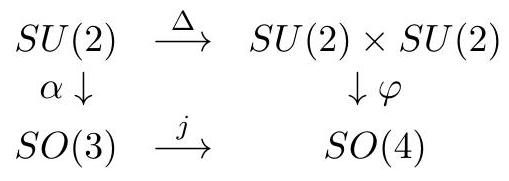
\includegraphics[max width=\textwidth, center]{2025_05_20_67e75debbfd3ba8ea587g-34}

Dabei ist $\Delta$ die Diagonalabbildung, $\Delta(A)=(A, A)$. Man zeigt leicht, dass $j$ injektiv ist. $H:=\operatorname{Bild}(j) \cong S O(3) \subseteq S O(4)$ ist eine Untergruppe. Ebenso ist $\varphi(S U(2) \times 1)=: G \cong S U(2) \subseteq S O(4)$ eine Untergruppe und sogar ein Normalteiler und $G \cap H=\{1\}$, denn $\varphi(A, 1)=\varphi(B, B) \Leftrightarrow \varphi\left(A^{-1} B, B\right)=$ id $\Leftrightarrow A=1$ und $B= \pm 1$.\\
Es ist $S O(4) / G \cong S O(3)$, da $\varphi(A, B)=\varphi\left(A, B^{-1}\right) \varphi(B, B)$ gilt, also $S O(4)=$ $G \cdot H$. Damit ist auch eine zweifache Überlagerung

$$
\begin{aligned}
S O(4) & \rightarrow S O(3) \times S O(3) \\
A & \rightarrow(\alpha \times \alpha) \varphi^{-1}(A)
\end{aligned}
$$

wohldefiniert. Dies ist die Darstellung von $S O(4)$ auf $\Lambda_{+}^{2} \mathbb{R}^{4} \oplus \Lambda_{-}^{2} \mathbb{R}^{4}=\Lambda^{2} \mathbb{R}^{4}$.

\section*{6.C Die symplektische Gruppe}
Die Quaternionen bilden einen Schiefkörper. $G L(n, \mathbb{H}):=\operatorname{Aut}_{\mathbb{H}}\left(\mathbb{H}^{n}\right)$ bezeichne die $\mathbb{H}$-linearen invertierbaren Abbildungen $\mathbb{H}^{n} \rightarrow \mathbb{H}^{n}$. Als komplexer Vektor ist $\mathbb{H}^{n}=\mathbb{C}^{n} \oplus \mathbb{C}^{n} \cdot J=\mathbb{C}^{2 n}$. Also ist

$$
\operatorname{End}_{\mathbb{H}} \mathbb{H}^{n}=\left\{A \in G L_{\mathbb{C}}\left(\mathbb{C}^{2 n} \mid A \circ J=J \circ A\right\}\right.
$$

und

$$
G L(n, \mathbb{H})=\left\{\left.\left(\begin{array}{cc}
A & -\bar{B} \\
B & A
\end{array}\right) \right\rvert\, A, B \in \operatorname{End}\left(\mathbb{C}^{n}\right)\right\}
$$

\subsection*{6.4 Definition und Notiz}
Die symplektische Gruppe ist

$$
\begin{aligned}
S p(n, \mathbb{H}) & =\left\{\left.\left(\begin{array}{cc}
A & -\bar{B} \\
B & A
\end{array}\right) \in U(2 n) \right\rvert\, A, B \in \operatorname{End}\left(\mathbb{C}^{n}\right)\right\} \\
& =\{A \in G L(n, \mathbb{H}) \mid\|A(X)\|=\|X\|\}
\end{aligned}
$$

wobei $\|X\|=\sum_{\nu} \operatorname{Spur}\left(\bar{X}_{\nu}^{T} \cdot X_{\nu}\right)$.

\subsection*{6.5 Bemerkung}
a) $S p(n)=\left\{S \in U(2 n) \mid S^{T} J S=J\right\}$ für $J=\left(\begin{array}{cc}0 & -\nVdash \\ \nVdash & 0\end{array}\right)$.\\
b) Die Liealgebra der symplektischen Gruppe ist

$$
S p(n)=\left\{\left.\left(\begin{array}{cc}
A & -\bar{B} \\
B & \bar{A}
\end{array}\right) \in G L(2 n, \mathbb{C}) \right\rvert\, \bar{A}^{T}=-A, B^{T}=B\right\}
$$

und folglich $\operatorname{dim} \operatorname{Sp}(n)=2 n^{2}+n$.

\section*{6.D Die pseudo-orthogonalen Gruppen}
Bekanntlich ist $S O^{\uparrow}(1, n-1) \cong \mathbb{R}^{n-1} \times S O(n-1)$. Die Liealgebra ist

$$
\begin{aligned}
s o(1, n-1) & =\left\{A \in \operatorname{End}\left(\mathbb{R}^{n}\right) \left\lvert\, \bar{A}^{T} \cdot\left(\begin{array}{cc}
1 & \\
& -\nVdash
\end{array}\right)=\left(\begin{array}{ll}
1 & \\
& -\nVdash
\end{array}\right) A\right.\right\} \\
& =\left\{\left.\left(\begin{array}{cc}
0 & t \\
b & c
\end{array}\right) \right\rvert\, b \in \mathbb{R}^{n-1}, c \in s o(n-1)\right\}
\end{aligned}
$$

\subsection*{6.6 Lemma}
Durch

$$
\begin{aligned}
\mathbb{R}^{1,3} & \rightarrow(\mathbb{H}(2, \mathbb{C}), \text { det }) \\
\left(\begin{array}{c}
t \\
x_{1} \\
x_{2} \\
x_{3}
\end{array}\right) & \mapsto\left(\begin{array}{cc}
t+x_{1} & x_{2}+i x_{3} \\
x_{2}-i x_{3} & t-x_{1}
\end{array}\right)
\end{aligned}
$$

ist eine Isometrie gegeben.\\
Beweis: Nachrechnen!

\subsection*{6.7 Satz}
Durch

$$
\begin{aligned}
\varphi: S L(2, \mathbb{C}) & \rightarrow S O^{\uparrow}(1,3) \\
A & \mapsto\left(X \mapsto\left(A X \bar{A}^{T}\right)\right.
\end{aligned}
$$

ist eine zweifache Überlagerung der Lorentzgruppe gegeben.\\
Beweis: Man rechnet leicht nach, dass $\varphi$ ein Gruppenhomomorphismus ist. Es ist $\operatorname{Ker} \varphi=\{ \pm \nVdash\}$, denn ist $A X \bar{A}^{T}=X$ für alle $X \in \mathbb{H}(2)$, also auch für $X=\nVdash$, so ist $\bar{A}^{T}=A^{-1}$, also $A X=X A$ für alle $X \in \mathbb{H}(2)$, also $A X=X A$ für alle $X \in M(2 \times 2, \mathbb{C})$, also ist $A=\lambda \nVdash$, also $A= \pm \nVdash$.\\
Die Abbildung $\varphi$ ist differenzierbar und $\left.d \varphi\right|_{1}$ ist ein Isomorophismus, also ist $\varphi$ ein lokaler Diffeomorphismus bei 1 , da $\varphi$ ein Homomorphismus ist. Da $S O^{\uparrow}(1,3)$ zusammenhängend ist, ist $\varphi$ auch surjektiv.

\subsection*{6.8 Bemerkung}
a) Die Einschränkung von $\varphi$ auf $S U(2)$ ist genau die adjungierte Darstellung und

$$
\varphi\left(\begin{array}{cc} 
\pm e^{s} & 0 \\
0 & \pm e^{-s}
\end{array}\right)=\left(\begin{array}{cccccc}
\cosh & 2 s & \sinh & 2 s & 0 & 0 \\
\sinh & 2 s & \cosh & 2 s & 0 & 0 \\
0 & & 0 & & 1 & 0 \\
0 & & 0 & & 0 & 1
\end{array}\right)
$$

b) Durch die Einschränkung auf reelle Einträge erhält man eine zweifache Überlagerung $S L(2, \mathbb{R}) \rightarrow S O^{\uparrow}(1,2)$.

\section*{6.E Spingruppen}
Weitere Gruppen, die eine wichtige Rolle in der Physik spielen, sind zweifache Überlagerungen der orthogonalen Gruppe. Wir haben bereits gesehen, dass die universelle Überlagerung einer Liegruppe wieder eine Liegruppe ist mit derselben Liealgebra. Für die orthogonalen Gruppen gilt:

$$
\begin{aligned}
\pi_{1}(S O(2)) & =\mathbb{Z} \\
\pi_{1}(S O(n)) & =\mathbb{Z}_{2} \text { für } n \geq 3 \\
\pi_{1}\left(S O^{\uparrow}(k, n-k)\right) & =\pi_{1}(S O(k)) \times \pi_{1}(S O(n-k))
\end{aligned}
$$

Wir sehen, dass für $S O(n), n \geq 3$ und $S O^{\uparrow}(1, r)$ mit $r \geq 3$ die zusammenhängende zweifache Überlagerung die universelle Überlagerung ist. Üblicherweise wird die Spingruppe als Teilmenge der Cliffordalgebra definiert, (ähnlich zu $s u(2) \subseteq \mathbb{H}$ ). Wir wollen Spingruppen nicht so ausführlich behandeln, deshalb definieren wir sie hier nur in Spezialfällen.

\subsection*{6.9 Definition}
Im Fall $n \geq 3$ ist $\operatorname{Spin}(n)$ bzw. $\operatorname{Spin}^{\uparrow}(1, n)$ die universelle Überlagerung von $S O(n)$ bzw. $S O^{\uparrow}(1, n)$.

\subsection*{6.10 Korollar}
$$
\begin{aligned}
\operatorname{Spin}(3) & =S U(2) \\
\operatorname{Spin}(4) & =S U(2) \times S U(2) \\
\operatorname{Spin}^{\uparrow}(1,3) & =S L(2, \mathbb{C})
\end{aligned}
$$

\subsection*{6.11 Bemerkung}
Außerdem gilt:

$$
\begin{aligned}
\operatorname{Spin}(5) & =S p(2) \\
\operatorname{Spin}(6) & =S U(4) \\
\operatorname{Spin}^{\uparrow}(1,2) & =S L(2, \mathbb{R}) \\
\operatorname{Spin}^{\uparrow}(1,5) & =S L(2, \mathbb{H}) \\
\operatorname{Spin}^{\uparrow}(2,2) & =S L(2, \mathbb{R}) \times S L(2, \mathbb{R})
\end{aligned}
$$

Die anderen Spingruppen sind nicht durch bekannte Gruppen beschreibbar. Jedenfalls gilt, dass $\operatorname{Spin}^{\uparrow}(k, n-k)$ bzw. $\operatorname{Spin}(n)$ eine komplexe irreduzible Darstellung der Dimension $2^{\left[\frac{n}{2}\right]-1}$ hat. Genaueres findet sich z.B. in Blaine Lawson, Marie-Louise Michelsohn, Spin Geometry, Princeton 1989, Kap.1.

\section*{7 Die Killing-Form}
Wir werden bald sehen, dass es oft wichtig ist, auf einer Liealgebra Adinvariante Skalarprodukte zu finden, d.h. Skalarprodukte, für die gilt

$$
\langle A d(g) X, A d(g) Y\rangle=\langle X, Y\rangle
$$

für alle $g \in G, X, Y \in \mathfrak{g}$.

\subsection*{7.1 Notiz}
a) Ist $B$ eine Ad-invariante Bilinearform auf $\mathfrak{g}$, so ist $B$ auch ad-invariant, d.h. es gilt

$$
\langle[X, A], B\rangle+\langle A,[X, B]\rangle=0
$$

für alle $A, B, X \in \mathfrak{g}$.\\
b) Ist $I \subseteq \mathfrak{g}$ ein Ideal und $B$ eine invariante symmetrische Bilinearform, so ist auch $I^{\perp}$ ein Ideal, denn für $A \in I, X \in \mathfrak{g}$ und $B \in I^{\perp}$ folgt

$$
\langle[X, B], A\rangle=\langle B,[X, A]\rangle=0
$$

Jede invariante symmetrische Bilinearform auf einer einfachen nicht abelschen Liealgebra ist nichtentartet.

\subsection*{7.2 Korollar}
Ist $\mathfrak{g}$ eine Liealgebra, $B$ eine ad-invariante symmetrische Bilinearform, $I$ ein Ideal, $I \cap I^{\perp}=\{0\}$, so ist $\mathfrak{g}=I \oplus I^{\perp}$.

\subsection*{7.3 Korollar}
Auf jeder (endlichdimensionalen) Liealgebra gibt es eine kanonische symmetrische invariante Bilinearform.

\subsection*{7.4 Lemma und Definition}
Ist $\rho: \mathfrak{g} \rightarrow \operatorname{End}(V)$ ein Liealgebren-Homomorphismus, so ist durch

$$
\kappa_{\rho}(X, Y)=\operatorname{tr}(\rho(X) \circ \rho(Y))
$$

eine symmetrische invariante Bilinearform auf $\mathfrak{g}$ definiert. Ist $\rho=\left.d \tau\right|_{1}$ für eine Darstellung $\tau: G \rightarrow G L(V)$, so ist $\kappa_{\rho}$ auch ad-invariant. $\kappa_{\text {ad }}=: \kappa$ heißt die Killingform.

Beweis: Offenbar ist $\kappa_{\rho}$ bilinear und symmetrisch, denn die Invarianz folgt durch direktes Nachrechnen:

$$
\begin{aligned}
& \kappa_{\rho}([X, Y], Z)+\kappa_{\rho}(Y,[X, Z]) \\
& =\operatorname{tr}(\rho(X) \circ \rho(Y) \circ \rho(Z)-\rho(Y) \rho(X) \rho(Z)) \\
& +\operatorname{tr}(\rho(Y) \circ \rho(X) \circ \rho(Z)-\rho(Y) \circ \rho(Z) \circ \rho(X))=0
\end{aligned}
$$

Für $\rho=\left.d \tau\right|_{1}$ gilt

$$
\begin{aligned}
\kappa_{\rho}(A d(g)(X), A d(g)(Y)) & =\operatorname{tr}\left(\left.\left.\tau(g) d \tau\right|_{1}(X) \tau\left(g^{-1}\right) \circ \tau(g) \circ d \tau\right|_{1}(Y) \tau\left(g^{-1}\right)\right) \\
& =\operatorname{tr}\left(\tau(g) \circ \rho(X) \circ \rho(Y) \circ \tau(g)^{-1}\right)=\kappa_{\rho}(X, Y)
\end{aligned}
$$

\subsection*{7.5 Beispiel}
a) Sei $\mathfrak{g}=s o(3)$. Dann ist

$$
\kappa=\left(\begin{array}{lll}
-2 & & \\
& -2 & \\
& & -2
\end{array}\right)
$$

bezüglich ( $E_{i j}$ ).\\
b) Sei $\mathfrak{g}=u(n)$. Dann ist $\kappa(X, Y)=2 n \operatorname{tr}(X Y)-2 \operatorname{tr}(X) \operatorname{tr}(Y)$.\\
c) Sei $\mathfrak{g}=s u(n)$. Dann ist $\kappa(X, Y)=2 n \operatorname{tr}(X Y)$.\\
c) Sei $\mathfrak{g}=s o(n)$. Dann ist $\kappa(X, Y)=(n-2) \operatorname{tr}(X Y)$.

\subsection*{7.6 Korollar}
Die Killingform auf einer einfachen, nichtabelschen Liealgebra ist nicht entartet.

\subsection*{7.7 Satz}
Eine Liealgebra ist genau dann halbeinfach, wenn ihre Killingform nicht entartet ist.

Beweis: Tits, Liesche Gruppen und Algebren.

\subsection*{7.8 Lemma}
Ist $\mathfrak{g}_{1} \oplus \mathfrak{g}_{2}=: \mathfrak{g}$ eine Summe einer halbeinfachen Liealgebra mit einer beliebigen Liealgebra, $B$ eine invariante Bilinearform auf $\mathfrak{g}$, so ist $\mathfrak{g}_{1} \perp \mathfrak{g}_{2}$ bezüglich $B$.

Beweis: Für einfache nichtabelsche Liealgebren $\mathfrak{g}_{1}$ gilt $\mathfrak{g}_{1}=\left[\mathfrak{g}_{1}, \mathfrak{g}_{1}\right]$ und für $X, Y \in \mathfrak{g}_{1}, Z \in \mathfrak{g}_{2}$ ist

$$
B([X, Y,], Z)=-B(X,[Y, Z])=0
$$

\subsection*{7.9 Korollar}
Ist $\mathfrak{g}_{0}$ eine abelsche Liealgebra und $\mathfrak{g}_{1} \ldots \mathfrak{g}_{p}$ nichtabelsche einfache Liealgebren, so sind die invarianten Bilinearformen auf $\mathfrak{g}_{0} \oplus \cdots \oplus \mathfrak{g}_{p}$ durch

$$
B\left(\left(X_{0} \ldots X_{p}\right),\left(Y_{0} \ldots Y_{p}\right)\right)=\sum_{i=0}^{p} B_{i}\left(X_{i}, Y_{i}\right)
$$

gegeben, wobei $B_{i}$ eine invariante Bilinearform auf $\mathfrak{g}_{i}$ ist.

\subsection*{7.10 Satz}
Die einzigen symmetrischen invarianten Bilinearformen auf einer einfachen nichtabelschen Liegruppe sind skalare Vielfache der Killingform.

Beweis: Sei $B$ eine weitere Bilinearform und $f_{B} \in \operatorname{End}(\mathfrak{g})$ der bezüglich der Killingform $\kappa$ gegebene symmetrische Endomorphismus

$$
\kappa\left(f_{B}(X), Y\right):=B(X, Y)
$$

Die Eigenräume von $f_{B}$ sind Ideale, denn ist $f_{B}(X)=\lambda X$, so ist für jedes $Z \in \mathfrak{g}$

$$
\begin{aligned}
\kappa\left(f_{B}([X, Y])-\lambda[X, Y], Z\right) & =B([X, Y], Z)-\lambda \kappa([X, Y], Z) \\
& =B(X,[Y, Z])-\lambda \kappa(X,[Y, Z]) \\
& =\kappa\left(f_{B}(X)-\lambda X,[Y, Z]\right)=0
\end{aligned}
$$

also ist $f_{B}=\lambda \operatorname{Id}$ für ein $\lambda \in \mathbb{R}$.

\subsection*{7.11 Bemerkung}
Ist $V$ ein komplexer Vektorraum und $f \in \operatorname{End}_{\mathbb{C}}(V)$, so ist

$$
t r_{\mathbb{R}} f=2 \operatorname{Re} t r_{\mathbb{C}} f
$$

\subsection*{7.12 Notiz}
Für $A, B \in \operatorname{su}(n)$ ist $\operatorname{tr}_{\mathbb{C}}(A \circ B)$ reell, also $\operatorname{tr}_{\mathbb{C}}(A \circ B)=2 \operatorname{tr}_{\mathbb{R}}(A \circ B)$, denn für $X \in s u(n)$ gilt $X=X_{1}+i X_{2}$ mit $X_{i} \in G L(n, \mathbb{R})$ und $X_{1}^{T}=-X_{1}, X_{2}^{T}=X_{2}$. Für $X$ symmetrisch und $Y$ schiefsymmetrisch ist aber

$$
\begin{aligned}
\operatorname{tr}_{\mathbb{C}}(X \circ Y) & =\operatorname{tr}_{\mathbb{C}}\left(Y^{t} \circ X^{t}\right) \\
& =\operatorname{tr}_{\mathbb{C}}(-Y \circ X) \\
& =-\operatorname{tr}_{\mathbb{C}}(X \circ Y)=0
\end{aligned}
$$

also ist für $A=A_{1}+i A_{2}, B=B_{1}+i B_{2}$

$$
\operatorname{tr}_{\mathbb{C}}(A \circ B)=\operatorname{tr}_{\mathbb{C}}\left(A_{1} \circ B_{1}-A_{2} \circ B_{2}\right)
$$

\subsection*{7.13 Lemma}
Für $A, B \in s u(n)$ ist $\operatorname{tr}_{\mathbb{R}}(\operatorname{ad}(A) \circ \operatorname{ad} B)=n \operatorname{tr}_{\mathbb{R}}(A \circ B)=2 n \operatorname{tr}_{\mathbb{C}}(A \circ B)$.\\
Beweis: Übung.\\
Weitergehende Aussage kann man treffen, wenn man eine andere Eigenschaft von Liealgebren betrachtet.

\subsection*{7.14 Definition}
Eine Liealgebra heißt kompakt, wenn sie Liealgebra einer einfach zusammenhängenden kompakten Liegruppe ist.

\subsection*{7.15 Beispiele}
a) $s o(2)=T_{1} S^{1}=T_{0} \mathbb{R}$ ist keine kompakte Liealgebra.\\
b) $s u(n)$ ist für jedes $n$ eine kompakte Liealgebra.

\subsection*{7.16 Satz}
\begin{enumerate}
  \item Eine Liealgebra ist genau dann kompakt, wenn ihre Killingform negativ definit ist.
  \item Die Liealgebra einer kompakten Liegruppe ist stets die Summe einer kompakten Liealgebra mit einer abelschen Liealgebra, genauer ist $\mathfrak{g}=$ $Z(\mathfrak{g}) \oplus[\mathfrak{g}, \mathfrak{g}]$
\end{enumerate}

\subsection*{7.17 Korollar}
Jede zusammenhängende kompakte Liegruppe ist isomorph zu einem Quotienten

$$
\left(T^{a} \times G_{1} \times \cdots \times G_{n}\right) / N,
$$

wobei $T^{a}=S^{1} \times \cdots \times S^{1}$ ein Torus und $G_{i}$ kompakte Untergruppen mit einfacher Liealgebra sind und $N$ eine diskrete Untergruppe von $T^{a} \times G_{1} \times \cdots \times G_{n}$ ist.

Die Beweise dieser Sätze sind wieder im Buch von Tits, Liesche Gruppen und Algebren, zu finden.

Die einfach zusammenhängenden Liegruppen mit einfachen kompakten Liealgebren sind:

\begin{center}
\begin{tabular}{lll}
Typ & Name & Dimension \\
$A_{r}, r \geq 1$ & $S U(r+1)$ & $r(r+2)$ \\
$B_{r}, r \geq 2$ & $\mathrm{Spin}(2 r+1)$ & $r(2 r+1)$ \\
$C_{r}, r \geq 3$ & $\mathrm{Sp}(r)$ & $r(2 r+1)$ \\
$D_{r}, r \geq 4$ & $\mathrm{Spin}(2 r)$ & $r(2 r-1)$ \\
$G_{2}$ & $G_{2}$ & 14 \\
$F_{r}$ & $F_{r}$ & 52 \\
$E_{6}$ & $E_{6}$ & 78 \\
$E_{7}$ & $E_{7}$ & 133 \\
$E_{8}$ & $E_{8}$ & 248 \\
\end{tabular}
\end{center}

Der Index $r$ gibt die höchste mögliche Dimension eines Torus an, der eingebettet werden kann.

\section*{8 Homogene Räume}
\subsection*{8.1 Definition}
a) Eine $G$-Aktion auf einer Mannigfaltigkeit $\phi: G \times M \rightarrow M$ heißt\\
(i) effektiv: $\Leftrightarrow\left(L_{g}=i d_{M} \Rightarrow g=1\right)$\\
(ii) einfach: $\Leftrightarrow\left(L_{g} x=x\right.$ für ein $\left.x \in M \Rightarrow g=1\right)$\\
(iii) transitiv: $\Leftrightarrow(\forall x, y \in M \exists g \in G: g x=y)$\\
iv) eigentlich, wenn die Abbildung $G \times M \rightarrow M \times M,(g, x) \mapsto(g x, x)$ eigentlich ist (vgl. Lee 9.12).\\
b) ( $M, \phi$ ) heißt homogener Raum, falls $G$ transitiv auf $M$ operiert.\\
c) Für $p \in M$ heisst

$$
G p:=\{\phi(g, p) \mid g \in G\}
$$

die Bahn von $p$ und

$$
G_{p}:=\{g \in G \mid g p=p\}
$$

die Isotropiegruppe (oder Standgruppe) von $p$.

\subsection*{8.2 Notiz}
a) Seien $p, q \in G x$ für ein $x \in M$. Dann ist $G_{p}$ konjugiert zu $G_{q}$, genauer: Ist $q=g p$, so ist $G_{q}=g G_{p} g^{-1}$.\\
b) Für jedes $x \in M$ ist $G_{x}$ eine abgeschlossene Untergruppe.

Wir benutzen die folgende

\subsection*{8.3 Proposition}
a) Ist $\phi: G \times M \rightarrow M$ eine eigentliche freie $G$-Aktion, dann ist $M / G$ eine topologische Mannigfaltigkeit (insbesondere Hausdorffsch!), vgl. Lee 9.15, 9.16.\\
b) Ist $H \subseteq G$ eine abgeschlossene Untergruppe, dann ist die kanonische $H$-Aktion auf $G$ eigentlich.

\subsection*{8.4 Satz}
a) Jede abgeschlossene Untergruppe einer Liegruppe ist eine Unterliegruppe.\\
b) Sei $H \subseteq G$ eine abgeschlossene Untergruppe. Auf $G / H$ existiert eine eindeutig bestimmte differenzierbare Struktur, sodass $\pi: G \rightarrow G / H$\\
eine lokal triviale Faserung mit typischer Faser $H$ und Strukturgruppe $H$ ist und

$$
G \times G / H \rightarrow G / H,\left(g,\left[g^{\prime}\right]\right) \mapsto\left[g g^{\prime}\right]
$$

eine differenzierbare Abbildung ist.\\
Beweis: a) Es genügt zu zeigen, dass lokal um 1 eine Untermannigfaltigkeitskarte existiert. Wir werden zeigen, dass sie durch exp gegeben ist.\\
Sei $W$ eine Normalumgebung der 1 in $G, V=\exp ^{-1}(W), \log :=\left(\left.\exp \right|_{V}\right)^{-1}$. Sei $A=\log (H \cap W)$. Wir nennen $X \in \mathfrak{g}$ tangential an $H$ (in 1), wenn eine Folge $\left(a_{k}\right)_{k \in \mathbb{N}}$ mit $a_{k} \in A$ und $\lim a_{k}=0$ existiert und eine Folge $\left(t_{k}\right)_{k \in \mathbb{N}}$ mit $t_{k} \in \mathbb{R}$ und $X=\lim _{k \rightarrow \infty} t_{k} a_{k}$.

$$
T A:=\{X \in \mathfrak{g} \mid X \text { tangential an } H\}
$$

Es gilt offenbar:\\
(i) $0 \in T A$.\\
(ii) Ist $X \in T A$, so ist $\mathbb{R} X \subseteq T A$.\\
(iii) $X$ ist invariant unter Verkleinern von $W$.

Es genügt, folgende Behauptungen zu zeigen:

\begin{enumerate}
  \item $\exp (T A) \subseteq H$, also $\exp (V \cap T A) \subseteq W \cap H$.
  \item $T A$ ist ein Untervektorraum.
  \item Nach Verkleinern von $W$ gilt: $\exp (V \cap T A) \supseteq W \cap H$.
\end{enumerate}

Ist 1)-3) gezeigt, so folgt, dass $\log \mid W$ eine Untermannigfaltigkeitskarte für $W \cap H$ ist.\\
Zu 1):\\
Sei $X \in T A$, also $X=\lim t_{k} a_{k}$. Da $a_{k} \in A$, ist $\exp \left(a_{k}\right) \in H$, also $\exp \left(\mathbb{Z} a_{k}\right) \in$ $H$ für alle $k \in \mathbb{N}$. Da $\lim a_{k}=0$, ist $\overline{\bigcup_{k=1}^{\infty} \mathbb{Z} a_{k}} \ni X$, also ist auch $\exp (X) \in H$, da $H$ abgeschlossen ist.

\section*{Zu 2):}
Seien $X, Y \in T A$. Dann ist $\exp (t X) \subseteq H$ und $\exp (t Y) \subseteq H$ (nach (ii)und 1)), also ist $\exp (t X) \cdot \exp (t Y) \in H$ für alle $t \in \mathbb{R}$. Sei

$$
\alpha: \mathbb{R} \rightarrow H \subseteq G, \alpha(t)=\exp (t X) \exp (t Y)
$$

Dann ist $\dot{\alpha}(0)=\lim _{t \rightarrow 0} \frac{\log (\alpha(t))}{t} \in T A$, da $\left.d \exp \right|_{0}=\mathrm{id}$, also $\dot{\alpha}(0)=\left.\frac{d}{d t}\right|_{t=0} \log \alpha(t)$. Andererseits ist

$$
\dot{\alpha}(0)=(\exp (t X) \dot{)}(0)+(\exp (t Y) \dot{)}(0)=X+Y,
$$

also $X+Y \in T A$.

Zu 3):\\
Angenommen nicht. Dann gäbe es eine Folge $\left(h_{k}\right)_{k \in \mathbb{N}}$ in $W \cap H$ mit $\lim _{k \rightarrow \infty} h_{k}=$ 1 und $h_{k} \notin \exp (V \cap T A)$ für alle $k$. Sei $\mathfrak{g}_{1}$ ein zu $T A$ komplementärer Unterraum in $\mathfrak{g}, \mathfrak{g}_{1} \oplus T A=\mathfrak{g}$. Sei oBdA $V$ so klein, dass

$$
\widetilde{\exp }:\left(T A \oplus \mathfrak{g}_{1}\right) \cap V \rightarrow W,(v, w) \mapsto \exp (v) \exp (w)
$$

ein Diffeomorphismus ist (möglich, da $\left.d \widetilde{\exp }\right|_{0}=\mathrm{id}$ ).\\
Sei $\widetilde{\exp }^{-1}\left(h_{k}\right)=: x_{k}+y_{k}$ mit $x_{k} \in T A, y_{k} \in \mathfrak{g}_{1}$. Dann ist $y_{k} \neq 0$ für alle $k$. Da $\exp \left(x_{k}\right) \exp \left(y_{k}\right)=h_{k} \in H$, ist $\exp \left(y_{k}\right) \in H$, also $y_{k} \in A$. Sei $\|\cdot\|$ eine Norm auf $\mathfrak{g}$, sodass $\bar{U}_{1}(0) \subseteq W$. OBdA existiert $\lim _{k \rightarrow \infty} \frac{y_{k}}{\left\|y_{k}\right\|}=: y \in \mathfrak{g}_{1} \cap T A=0$. Widerspruch!\\
b) Mit der Quotiententopologie ist $G / H$ in kanonischer Weise ein Hausdorffraum, $G \rightarrow G / H$ stetig und offen (Lee: 9.14-9.16).

Existiert eine differenzierbare Struktur wie gefordert, so ist sie eindeutig, denn dann hat $\pi$ lokal ein Rechtsinverses $\sigma$.\\
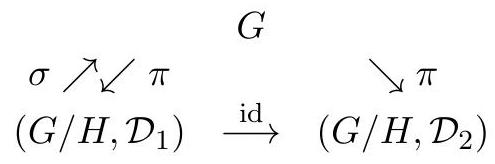
\includegraphics[max width=\textwidth, center]{2025_05_20_67e75debbfd3ba8ea587g-44}

Sind also $\mathcal{D}_{1}$ und $\mathcal{D}_{2}$ differenzierbare Strukturen wie gefordert, $\sigma_{j}: U \rightarrow G / H$ differenzierbare Schnitte bezüglich $\mathcal{D}_{j}$, so sind id $\mid U=\pi \circ \sigma_{1}$ und id $\mid U=\pi \circ \sigma_{2}$ beide differenzierbar.

Existenz: Sei $W \subseteq G$ eine Normalumgebung der 1 in $G$ und $V=\exp ^{-1}(W) \subseteq \mathfrak{g}$ und $\mathfrak{m}$ ein Komplement zu $\mathfrak{h} \subseteq \mathfrak{g}$, also $\mathfrak{g}=\mathfrak{m} \oplus \mathfrak{h}$. Sei $W_{\mathfrak{m}}=\mathfrak{m} \cap V$ und $s: W_{\mathfrak{m}} \rightarrow G, s(v)=\exp (v)$, also $s(0)=1,\left.d s\right|_{0}(\mathfrak{m}) \oplus \mathfrak{h}=\mathfrak{g}$.

Behauptung 1: Nach Verkleinern von $W_{\mathfrak{m}}$ ist $\phi: W_{\mathfrak{m}} \times H \rightarrow G,(v, h) \mapsto s(v) h$ ein Diffeomorphismus auf eine offene Teilmenge von $G$, also eine Umgebung von $H$.

Beweis von Behauptung 1: $d \phi_{(0,1)}$ ist ein Isomorphismus, also ist für $W_{\mathfrak{m}}$ klein genug $d \phi_{(x, 1)}$ ein Isomorphismus für alle $x \in W_{\mathfrak{m}}$, also ist $d \phi_{(x, h)}=d R_{h} \circ d \phi_{(x, 1)}$ ein Isomorphismus für alle $(x, h) \in W_{\mathfrak{m}} \times H$. Zu zeigen bleibt, dass $W_{\mathfrak{m}}$ so verkleinert werden kann, dass $\phi$ injektiv ist.\\
Angenommen nicht. Seien $\left(a_{i}\right),\left(b_{i}\right)$ Folgen in $W_{\mathfrak{m}}$ mit $\lim a_{i}=\lim b_{i}=0$ und $h_{i}, k_{i}$ Folgen in $H$ mit $s\left(a_{i}\right) h_{i}=s\left(b_{i}\right) k_{i}$, also $s\left(a_{i}\right)=s\left(b_{i}\right) k_{i} h_{i}^{-1}$ und folglich wegen $\lim s\left(a_{i}\right)=\lim s\left(b_{i}\right)=1$ auch $\lim k_{i} h_{i}^{-1}=1$. Lokal bei $(0,1)$ ist $\phi$ ein Diffeomorphismus, also folgt $a_{i}=b_{i}$ und $k_{i}=h_{i}$.\\
Also ist

$$
\psi: W_{\mathfrak{m}} \rightarrow U:=\pi\left(\phi\left(W_{\mathfrak{m}} \times H\right)\right) \subseteq G / H, v \mapsto[s(v)]
$$

eine stetige offene Bijektion, also ist ( $U, \psi^{-1}$ ) eine topologische Karte um [1]. $G$ operiert stetig auf $G / H$, also ist $\mathfrak{A}=\left\{g U \mid \psi^{-1} \circ L_{g-1}\right\}$ ein topologischer Atlas für $G / H$.

Behauptung 2: Dies ist eine differenzierbare Struktur, d.h. die Kartenwechsel sind Diffeomorphismen.

Beweis von Behauptung 2: Sei $\varphi_{g}: W_{\mathfrak{m}} \rightarrow g U \subseteq G / H, v \mapsto[g s(v)]$.\\
Sei

$$
w_{g^{\prime} g}=\varphi_{g^{\prime}}^{-1} \circ \varphi_{g}: \varphi_{g}^{-1}\left(g U \cap g^{\prime} U\right) \rightarrow \varphi_{g^{\prime}}^{-1}\left(g U \cap g^{\prime} U\right)
$$

Dann ist

$$
\begin{aligned}
{\left[g^{\prime} s\left(w_{g^{\prime} g}(v)\right)\right]=[g s(v)] } & \Leftrightarrow \exists h \in H: g^{\prime} s\left(w_{g^{\prime} g}(v)\right) h=g s(v) \\
& \Leftrightarrow s\left(w_{g^{\prime} g}(v)\right) h=g^{\prime-1} g s(v)
\end{aligned}
$$

Da die linke Seite in $\pi^{-1}(U)=\phi\left(W_{\mathfrak{m}} \times H\right)$ ist, ist also:

$$
w_{g^{\prime} g}(v)=p r_{1} \phi^{-1}\left(g^{\prime-1} g s(v)\right)
$$

also ist $w_{g^{\prime} g}$ differenzierbar.\\
Existenz lokaler Rechtsinverser: Die Abbildung $L_{g} \circ s \circ \varphi_{g}^{-1}: g U \rightarrow G,[g s(v)] \mapsto$ $g s(v)$ ist ein lokales Rechtsinverses zu $G \rightarrow G / H$, also ist $G \rightarrow G / H$ ein $H$ Prinzipalbündel.\\
Die Abbildung $G \times G / H \rightarrow G / H$ ist differenzierbar, denn $G \rightarrow G / H$ besitzt lokale Rechtsinverse $\sigma$, also folgt dies aus der Differenzierbarkeit der $G$-Aktion auf $G$

$$
\begin{array}{ccc}
G \times G & \longrightarrow & G \\
d x \sigma \uparrow \downarrow & & \downarrow \\
G \times G /\left.H\right|_{U} & \longrightarrow & G / H
\end{array}
$$

\subsection*{8.5 Lemma}
Sei $\phi: G \times M \rightarrow M$ eine $G$-Aktion.\\
a) Für jedes $p \in M$ ist die Bahnabbildung $\alpha_{p}: G / G_{p} \rightarrow M,[g] \mapsto g p$ eine injektive äquivariante Immersion mit Bild $G p$.\\
b) Ist $G p$ kompakt oder $M$ ein homogener Raum, so ist $G p$ eine Untermannigfaltigkeit von $M$ und $\alpha_{p}: G / G_{p} \rightarrow G p$ ein Diffeomorphismus.

Beweis: a) Es genügt zu zeigen, dass $\left.d f\right|_{[1]}$ für $f=\alpha_{p}$ injektiv ist. Sei $v \in$ $T_{1}\left(G / G_{x}\right)$ mit $\left.d f\right|_{1}(v)=0$. Sei $w \in G$ mit $d \pi(w)=v$. Dann ist $\left.d f\right|_{1} \circ d \pi(w)=0$, also $\left.\frac{d}{d t}\right|_{t=0} \exp (t w) x=0$, also

$$
0=\left.\frac{d}{d t}\right|_{t=0} \exp \left(t_{0} w\right) \exp \left(t w-t_{0} w\right) x=\left.d L_{\exp \left(t_{0} w\right)} \cdot \frac{d}{d t}\right|_{t=t_{0}} \exp (t w) x
$$

also ist $\frac{d}{d t} \exp (t w) x \equiv 0$, also ist $\exp (t w) x=x$ für alle $t$, also $\exp (t w) \in G_{x}$, also $w \in \mathfrak{g}_{x}:=T_{1} G_{x}$, also $v=0$.\\
b) Die Abbildung hat konstanten Rang, also folgt die Behauptung aus dem Rangsatz (z.B. Lee, 7.15)

\subsection*{8.6 Beispiele}
a) $S^{n} \cong S O(n+1) / S O(n)$, denn $S O(n+1)$ wirkt transitiv auf $S^{n}$ und

$$
G_{e_{1}}=\left\{\left.\left(\begin{array}{cccc}
1 & 0 & \ldots & 0 \\
0 & & & \\
\vdots & & & \\
0 & & A &
\end{array}\right) \right\rvert\, A \in S O(n)\right\}=\{1\} \times S O(n) \cong S O(n)
$$

Ebenso ist $S^{n}=O(n+1) / O(n)$ und $S^{2 n-1}=U(n) / U(n-1)$.\\
b) $\mathbb{R} P^{n}=S O(n+1) / S(O(n) \times O(1))$ mit

$$
S(A \times B)=\{X \in A \times B \mid \operatorname{det} X=1\}
$$

denn $\mathbb{R} P^{n}=S^{n} / \pm 1$, also operiert $S O(n+1)$ transitiv auf $\mathbb{R} P^{n}$ und

$$
G_{\left[e_{1}\right]}=\{1\} \times S O(n) \cup\{-1\} \times(O(n) \backslash S O(n))
$$

Ebenso ist $\mathbb{C} P^{n}=S U(n+1) / S(U(1) \times U(n))$.\\
c) Sei $\mathbb{C}_{+}=\{z \in \mathbb{C} \mid \operatorname{Im} z>0\}$.

$$
\begin{aligned}
S L(2, \mathbb{R}) \times \mathbb{C}_{+} & \rightarrow \mathbb{C}_{+} \\
\left(\left(\begin{array}{ll}
a & b \\
c & d
\end{array}\right), z\right) & \mapsto \frac{a z+b}{c z+d}
\end{aligned}
$$

ist wohldefiniert, denn $c z+d \neq 0$, da $\operatorname{Im} z \neq 0$ und

$$
\operatorname{Im}(A z)=\frac{\operatorname{Im}(z)}{|c z+d|^{2}}>0
$$

und $A(B z)=(A B) z$. Ist $z=: x+i y$, so ist

$$
z=\left(\begin{array}{cc}
\sqrt{y} & \frac{x}{\sqrt{y}} \\
0 & \frac{1}{\sqrt{y}}
\end{array}\right) \cdot i
$$

Also ist die Wirkung transitiv. Die Standgruppe von $i$ ist $S O(2)$, denn

$$
\begin{aligned}
& \frac{a i+b}{c i+d}=i \\
\Leftrightarrow & a i+b=d i-c \\
\Leftrightarrow & a=d \wedge b=-c,
\end{aligned}
$$

also

$$
G_{i}=\left\{\left.\left(\begin{array}{cc}
a & -b \\
b & a
\end{array}\right) \right\rvert\, a^{2}+b^{2}=1\right\}=S O(2)
$$

also ist $\mathbb{C}_{+}=S L(2, \mathbb{R}) / S O(2)$.\\
d)

$$
\begin{aligned}
H^{n} & =\left\{x \in \mathbb{R}^{n+1} \mid-x_{0}^{2}+x_{1}^{2}+\cdots+x_{n}^{2}=-1, x_{0}>0\right\} \\
& =\mathcal{L}^{\uparrow}(1, n) / S O(n) .
\end{aligned}
$$

e) Da Darstellungen der Spingruppen durch $\pi$ : Spin $\rightarrow S O$ gegeben sind, gilt auch

$$
S^{n}=\operatorname{Spin}(n+1) / \operatorname{Spin}(n),
$$

also

$$
S^{2}=S U(2) / S O(2)=S^{3} / S^{1} \quad \text { Hopf-Faserung }
$$

und

$$
H^{n}=\operatorname{Spin}^{\uparrow}(1, n) / \operatorname{Spin}(n)
$$

also

$$
\begin{aligned}
H^{3} & =S L(2, \mathbb{C}) / S U(2) \\
H^{2} & =S L(2, \mathbb{R}) / S^{1}
\end{aligned}
$$

f) Auf dem Raum $\operatorname{Sym}_{+}^{2}\left(\mathbb{R}^{n}\right)$ der positiv definiten symmetrischen reellen $n \times n$ Matrizen ist eine transitive $G L(n, \mathbb{R})$-Aktion durch $(A, X) \mapsto$ $A X \bar{A}^{t}$ gegeben. Damit ist

$$
\operatorname{Sym}_{+}^{2}\left(\mathbb{R}^{n}\right)=G L(n, \mathbb{R}) / O(n)
$$

g) $\mathcal{L}$ bezeichne die Menge der Gitter, d.h. der Untergruppen in $\mathbb{R}^{2}$, die durch eine Basis $\left(v_{1}, v_{2}\right)$ in $\mathbb{R}^{2}$ erzeugt werden. Dann ist

$$
\mathcal{L}=G L(2, \mathbb{R}) / G L(2, \mathbb{Z})
$$

$\mathcal{L}_{1} \subseteq \mathcal{L}$ sei die Menge der unimodularen Gitter, also der Gitter mit $\operatorname{vol}\left(\operatorname{Spat}\left(v_{1}, v_{2}\right)\right)=1$. Dann ist $\mathcal{L}_{1}=S L(2, \mathbb{R}) / S L(2, \mathbb{Z})$. $\mathcal{L}_{1}$ ist homöomorph zum Komplement des Kleeblattknotens in $\mathbb{R}^{3}$ (vgl. Milnor, KTheorie).\\
h) Der Raum $J_{n}$ der komplexen Strukturen auf $\mathbb{R}^{2 n}$, die ein Skalarprodukt erhalten,

$$
J_{n}=\left\{A \in O(2 n) \mid A^{2}=-i d\right\}
$$

ist ein homogener Raum

$$
J_{n}=O(2 n) / U(n)
$$

i) $\mathcal{H}_{n}=\operatorname{Sp}(2 n) / U(n)$ ist der Raum der komplexen Strukturen, die eine alternierende Biliniarform erhalten. $\mathcal{H}_{n}$ heiße Siegelsche Halbebene.\\
j) Ist ( $M, g$ ) eine Riemannsche Mannigfaltigkeit, dann ist die Gruppe der Isometrien $f:(M, g) \rightarrow(M, g)$ eine Liegruppe.\\
Es gilt: $\operatorname{Isom}(M, g) \subseteq O\left(T_{x_{0}} M, T_{f\left(x_{0}\right)} M\right)$ für ein $x_{0} \in M$, falls $M$ vollständig und zusammenhängend ist. Denn ist $x_{0} \in M$, so ist $f \in \operatorname{Isom}(M, g)$ vollständig bestimmt durch $f\left(x_{0}\right)$ und $d f_{x_{0}}: T_{x_{0}} M \rightarrow T_{f\left(x_{0}\right)} M$, da Isometrien Geodätische auf Geodätischen abbilden. Eine Riemannsche Mannigfaltigkeit ( $M, g$ ) heißt symmetrisch, falls für jedes $x \in M$ eine Isometrie $f_{x}$ existiert mit $\left.d f_{x}\right|_{x}=-1$. Symmetrische Mannigfaltigkeiten sind vollständig.\\
Jede symmetrische Riemannsche Mannigfaltigkeit ist homogen, denn sind $x, y \in M$, dann gibt es eine Geodätische mit $\gamma(-1)=x, \gamma(1)=$ $y, \gamma(0)=: z$, also $f_{z}(x)=y$.\\
Symmetrische Räume können durch Krümmungseigenschaften beschrieben werden und sind vollständig klassifiziert (vgl. Helgason, symmetric spaces).

\subsection*{8.7 Bemerkung}
Wir wollen nun das Tangentialbündel von $G / H$ beschreiben. Ist $\mathfrak{m}$ ein zu $\mathfrak{h}$ komplementärer Unterraum in $\mathfrak{g}$, so ist offenbar die Einschränkung von

$$
\left.d \pi\right|_{1}: \mathfrak{g} \rightarrow T_{[1]}(G / H)
$$

auf $\mathfrak{m}$ ein Isomorphismus, denn Ker $\left.d \pi\right|_{1}=\mathfrak{h}$. Ist eine Zerlegung $\mathfrak{g}=\mathfrak{h} \oplus \mathfrak{m}$ gewählt, so fassen wir $T_{[1]} G / H=\mathfrak{m}$ auf.

\subsection*{8.8 Beispiel}
$G r_{k}(\mathbb{R})=O(n) /(O(k) \times O(n-k))$. Wegen

$$
o(n)=(o(k) \times o(n-k)) \oplus\left\{\left.\left(\begin{array}{cc}
0 & A \\
-A^{T} & 0
\end{array}\right) \right\rvert\, A \in(M(k \times(n-k))\}\right.
$$

ist also

$$
T_{[1]}\left(G r_{k}\left(\mathbb{R}^{n}\right)\right) \cong M(k \times(n-k))
$$

Besonders einfach ist das Tangentialbündel zu beschreiben, wenn der homogene Raum reduktiv ist.

\subsection*{8.9 Definition}
Ein homogener Raum $M=G / H$ heißt reduktiv, falls es einen Untervektorraum $\mathfrak{m} \subseteq \mathfrak{g}$ gibt mit

$$
\mathfrak{g}=\mathfrak{m} \oplus \mathfrak{h} \text { und } \operatorname{Ad}(H) \mathfrak{m} \subseteq \mathfrak{m}
$$

\subsection*{8.10 Bemerkung}
a) Ist $G / H$ reduktiv, so gilt auch $[\mathfrak{h}, \mathfrak{m}] \subseteq \mathfrak{m}$ und ist $H$ zusammenhängend und $[\mathfrak{h}, \mathfrak{m}] \subseteq \mathfrak{m}$, so ist $G$ reduktiv (vgl. 5.8).\\
b) Existiert auf $\mathfrak{g}$ eine positiv definite invariante symmetrische Bilinearform $B$ und ist $H$ zusammenhängend, so ist $M$ reduktiv, denn $\mathfrak{g}=\mathfrak{h} \oplus \mathfrak{h}^{\perp}$ ist eine ad-invariante Zerlegung, da

$$
B(X,[Y, Z])=-B([X, Y], Z)=0
$$

für alle $X, Y \in \mathfrak{h}$ und $Z \in \mathfrak{h}^{\perp}$ und folglich ist auch $\operatorname{Ad}(H) \mathfrak{m} \in \mathfrak{m}$.

\subsection*{8.11 Definition}
Ist $L_{g}: G / H \rightarrow G / H$ die Linksmultiplikation, so heißt die Abbildung

$$
\begin{aligned}
\rho: H & \rightarrow \operatorname{End}\left(T_{[1]} G / H\right) \\
h & \left.\mapsto d L_{h}\right|_{1}
\end{aligned}
$$

die Isotropiedarstellung $\rho$ von $H$.

\subsection*{8.12 Satz}
Ist $M$ ein reduktiver homogener Raum, und identifiziert man $T_{[1]}(G / H) \cong \mathfrak{m}$, so gilt $\rho=\left.\operatorname{Ad}\right|_{H}: H \rightarrow \operatorname{End}(\mathfrak{m})$.

Beweis: $\mathfrak{g}=\mathfrak{h} \oplus \mathfrak{m}$ mit $\operatorname{Ad}(H) \mathfrak{m} \subseteq \mathfrak{m}$. Für $X \in \mathfrak{m}, h \in H$ gilt

$$
\begin{aligned}
\left.d \pi\right|_{1}(\operatorname{Ad}(h) X) & =\left.\frac{d}{d t}\right|_{t=0}[\exp (t \operatorname{Ad}(h) X)] \\
& =\left.\frac{d}{d t}\right|_{t=0}[\operatorname{konj}(h) \exp (t X)] \\
& =\left.\frac{d}{d t}\right|_{t=0}\left[L_{h}(\exp (t X))\right] \\
& =\rho(h)\left(\left.d \pi\right|_{1}(X)\right)
\end{aligned}
$$

\subsection*{8.13 Beispiel}
$S^{n} \cong S O(n+1) / S O(n)$ ist ein reduktiver homogener Raum. Es ist

$$
H:=G_{e_{1}}=\left\{\left.\left(\begin{array}{cccc}
1 & 0 & \ldots & 0 \\
0 & & & \\
\vdots & & A &
\end{array}\right) \right\rvert\, A \in S O(n)\right\}
$$

und

$$
\alpha_{e_{i}}: S O(n+1) / S O(n) \rightarrow S^{n},[A] \mapsto A e_{1}
$$

Also ist $\mathfrak{g}=s o(n+1)$ und $\mathfrak{h}=0 \oplus s o(n)$. Ein Komplement von $\mathfrak{h} \subseteq \mathfrak{g}$ ist offenbar durch

$$
\mathfrak{m}=\left\{\left.\left(\begin{array}{cc}
0 & -b^{T} \\
b & 0
\end{array}\right) \right\rvert\, b \in \mathbb{R}^{n}\right\} \cong \mathbb{R}^{n}
$$

gegeben. Sei

$$
f: \mathbb{R}^{n} \rightarrow \mathfrak{m}, b \mapsto\left(\begin{array}{cc}
0 & -b^{T} \\
b & 0
\end{array}\right)
$$

der kanonische Isomorphismus. Dann ist für $b \in \mathbb{R}^{n}, h \in S O(n)$ und $\tilde{h}=\left(\begin{array}{ll}1 & 0 \\ 0 & h\end{array}\right)$ wie man leicht nachrechnet

$$
\operatorname{Ad}(\tilde{h})(f(b))=f(h b) \in \mathfrak{m}
$$

Außerdem ist

$$
\kappa\left(f\left(b_{1}\right), f\left(b_{2}\right)\right)=\frac{1}{2} \operatorname{tr}\left(f\left(b_{1}\right) f\left(b_{2}\right)\right)=-\left\langle b_{1}, b_{2}\right\rangle
$$

\subsection*{8.14 Bemerkung}
Nicht jeder homogene Raum ist reduktiv. Sei

$$
G=G L(2, \mathbb{R}), H=\left\{\left.\left(\begin{array}{cc}
1 & a \\
0 & b
\end{array}\right) \right\rvert\, a \in \mathbb{R}, b>0\right\}
$$

Dann ist

$$
\mathfrak{g}=g \ell(2, \mathbb{R}) \text { und } \mathfrak{h}=\left\{\left.\left(\begin{array}{ll}
0 & x_{1} \\
0 & x_{2}
\end{array}\right) \right\rvert\, x_{i} \in \mathbb{R}\right\} \cong \mathbb{R}^{2}
$$

Ist $\mathfrak{m} \subset g \ell(2, \mathbb{R})$ ein zu $\mathfrak{h}$ komplementärer Unterraum, so existiert in $\mathfrak{m}$ jedenfalls eine Matrix $\left(\begin{array}{ll}a & b \\ c & d\end{array}\right) \in g \ell(2, \mathbb{R})$ mit $c \neq 0$. Es ist

$$
\left[\left(\begin{array}{ll}
0 & 1 \\
0 & 0
\end{array}\right),\left(\begin{array}{ll}
a & b \\
c & d
\end{array}\right)\right]=\left(\begin{array}{cc}
-c & a-d \\
0 & c
\end{array}\right)
$$

und

$$
\left[\left(\begin{array}{cc}
0 & 1 \\
0 & 0
\end{array}\right),\left(\begin{array}{cc}
-c & a-d \\
0 & c
\end{array}\right)\right]=\left(\begin{array}{cc}
0 & -2 c \\
0 & 0
\end{array}\right) \in \mathfrak{h} .
$$

Ist also $\mathfrak{g}=\mathfrak{m}+\mathfrak{h}$ und $[\mathfrak{h}, \mathfrak{m}] \subseteq \mathfrak{m}$, so ist $\mathfrak{m} \cap \mathfrak{h} \neq\{0\}$.

\subsection*{8.15 Übungsaufgaben}
\begin{enumerate}
  \item Sei $G$ eine Liegruppe, $H \subseteq G$ eine abgeschlossene Untergruppe. Zeigen Sie, dass die Menge der $G$-äquivarianten Abbildungen $G / H \rightarrow G / H$ eine Liegruppe ist und differenzierbar auf $G / H$ operiert.
  \item Es bezeichne $C:=\left\{x \in \mathbb{R}^{1, n+1} \mid\langle x, c\rangle_{1, n+1}=0\right\}$ den Lichtkegel im $(n+2)$ - dimensionalen Minkowski-Raum und $P C:=\{\mathbb{R} x \mid x \in C \backslash\{0\}\}$ seine Projektivierung.\\
a) Zeigen Sie, dass $P C$ diffeomorph zur Sphäre $S^{n}$ ist.\\
b) Zeigen Sie, dass die pseudo-orthogonale Gruppe $O(1, n+1)$ transitiv auf $P C$ wirkt. Bestimmen Sie den Stabilisator des Punktes $\mathbb{R}(1,0, \ldots, 0,1) \in P C$.
\end{enumerate}

\section*{9 G-Vektorraumbündel}
\subsection*{9.1 Definition}
a) Ein Vektorraumbündel $E \rightarrow M$ heißt ein $G$-Vektorraumbündel, falls $M$ und $E G$-Mannigfaltigkeiten sind, sodass die $G$-Aktionen verträglich sind, d.h.\\
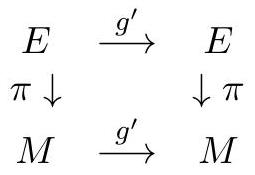
\includegraphics[max width=\textwidth, center]{2025_05_20_67e75debbfd3ba8ea587g-51}\\
kommutiert und für jedes $p \in M$ ist die Einschränkung der $G$-Aktion auf $E_{f}$ eine lineare Abbildung

$$
L_{g}: E_{p} \rightarrow E_{g p} .
$$

b) Ist $s \in \Gamma E$ ein Schnitt in einem $G$-Vektorraumbündel, so definiert man für $g \in G$

$$
\left(g_{*} s\right) \in \Gamma E
$$

durch

$$
(g s)(x)=g s\left(g^{-1} x\right)
$$

Ein Schnitt heißt äquivariant, falls $g_{*} s=s$ gilt.

\subsection*{9.2 Beispiel}
Sei $M$ eine $G$-Mannigfaltigkeit. Dann ist $T M$ ein $G$-Vektorraumbündel, denn für jedes $g \in G$ und $x \in M$ ist

$$
\left.d L_{g}\right|_{x}: T_{x} M \rightarrow T_{g_{x}} M
$$

eine lineare Abbildung. Auch $T^{*} M$ ist ein $G$-Vektorraumbündel, denn

$$
\begin{aligned}
G \times T^{*} M & \rightarrow T^{*} M \\
(g, \alpha) & \mapsto L_{g^{-1}}^{*} \alpha=\left.\alpha \circ d L_{g^{-1}}\right|_{g x}
\end{aligned}
$$

ist eine $G$-Aktion auf $T^{*} M$, die fasernweise linear ist. Ebenso sind $\operatorname{Sym}^{2} T^{*} M$, $\mathrm{Alt}^{k} T M G$-Vektorraumbündel. Die äquivarianten Schnitte sind dann genau die $G$-invarianten Vektorfelder, Differenzialformen oder Metriken.

\subsection*{9.3 Definition}
Sind $E_{1} \rightarrow G / H$ und $E_{2} \rightarrow G / H G$-Vektorraumbündel, so heißt ein Vektorraumbündelisomorphismus $f$ ein $G$-Vektorraumbündelisomorphismus, falls $f(g e)=g \cdot f(e)$ gilt für alle $g \in G, e \in E_{1}$.

\subsection*{9.4 Satz und Definition}
Ist $\rho: H \rightarrow \operatorname{End}(V)$ eine Darstellung, so existiert auf

$$
G \times{ }_{\rho} V:=G \times V / \sim \operatorname{mit}(g, v) \sim\left(g h, h^{-1} v\right):=\left(g h, \rho\left(h^{-1}\right) v\right)
$$

eine kanonische differenzierbare Struktur, sodass $G \times{ }_{\rho} V \rightarrow G / H$ eine surjektive Submersion ist. Dann ist $G \times{ }_{\rho} V$ ein $G$-Vektorraumbündel mit der $G$-Aktion

$$
\begin{aligned}
G \times\left(G \times{ }_{\rho} V\right) & \rightarrow G \times{ }_{\rho} V \\
\left(g_{1},\left[g_{2}, v\right]\right) & \mapsto\left[g_{1} g_{2}, v\right]
\end{aligned}
$$

Beweis: Sei $[g, v] \in G \times \rho V$. Sei $(U, \varphi)$ eine $H$-Bündelkarte für $G \rightarrow G / H$, also $U$ eine Umgebung von $[g]$ in $G / H$ und $\varphi: \pi^{-1}(U) \rightarrow U \times H$ eine $H$ äquivariante Abbildung, sodass

$$
\begin{array}{ccc}
\pi^{-1}(U) & \xrightarrow{\varphi} & U \times H \\
\pi \searrow & & \swarrow p r
\end{array}
$$

kommutiert.\\
Sei $\varphi(g)=:(\pi(g), \tilde{\varphi}(g))$. Dann ist $\tilde{\varphi}(g h)=\tilde{\varphi}(g) h$.\\
Sei $W:=\left\{[g, v] \in G \times_{\rho} V \mid[g] \in U, v \in V\right\} \subseteq G \times_{H} V$.

$$
\psi_{\varphi}: W \rightarrow U \times V, \quad[g, v] \mapsto(\pi(g), \rho(\tilde{\varphi}(g)) v) .
$$

Dann ist $\psi_{\varphi}$ wohldefiniert, denn

$$
\begin{aligned}
\psi_{\varphi}\left(\left[g h, \rho\left(h^{-1}\right) v\right]\right) & =\left(\pi(g h), \rho(\tilde{\varphi}(g h)) \rho\left(h^{-1}\right) v\right) \\
& =\left(\pi(g), \rho(\tilde{\varphi}(g)) \rho(h) \rho\left(h^{-1}\right) v\right) \\
& =(\pi(g), \rho(\tilde{\varphi}(g)) v) \\
& =\psi([g, v])
\end{aligned}
$$

Die Abbildung $\psi_{\varphi}$ ist injektiv und surjektiv, denn

$$
\psi_{\varphi}\left(\left[g, \rho(\tilde{\varphi}(g))^{-1} v\right]\right)=([g], v)
$$

also ist $\psi$ ein Homöomorphismus. Die differenzierbare Struktur auf $G \times{ }_{\rho} V$ wird durch die Forderung, dass $\psi_{\varphi}$ differenzierbar ist, defniert. Dies ist wohldefiniert, denn sind $\left(U, \varphi_{1}\right),\left(U, \varphi_{2}\right)$ verschiedene $H$-Bündelkarten, so ist $\psi_{\varphi_{1}} \circ \psi_{\varphi_{2}}^{-1}$ ein Diffeomorphismus.

Der folgende Satz zeigt, dass im Wesentlichen jedes $G$-Vektorraumbündel von dieser Form ist.

\subsection*{9.5 Satz}
Ist $E \rightarrow G / H$ ein $G$-Vektorraumbündel $V=E_{[1]}, \rho: H \rightarrow \operatorname{End}\left(E_{[1]}\right)$ die durch die Einschränkung der $G$-Aktion auf $H$ gegebene Darstellung, so ist

$$
f: G \times_{\rho} E_{[1]} \rightarrow E,[g, e] \mapsto g e
$$

ein $G$-Vektorraumbündelisomorphismus.\\
Beweis: Übungsaufgabe!

\subsection*{9.6 Korollar}
Ist $M=G / H$ ein homogener Raum und $\rho$ die Isotropiedarstellung, so ist $T M=G \times{ }_{\rho} T_{[1]} M$. Ist $M$ reduktiv, $\mathfrak{g}=\mathfrak{h} \oplus \mathfrak{m}$, so ist $T M=G \times{ }_{\mathrm{Ad}} \mathfrak{m}$. Der Isomorphismus ist durch

$$
G \times_{\mathrm{Ad}} \mathfrak{m} \rightarrow T M,\left.[g, X] \mapsto d L_{g}\right|_{1}(X)
$$

wohldefiniert.

\subsection*{9.7 Beispiel}
$T S^{n}=S O(n+1) \times_{S O(n)} \mathbb{R}^{n}$. Der Isomorphismus $S O(n+1) \times_{S O(n)} \mathbb{R}^{n} \rightarrow T S^{n}$ ist durch $[A, v] \mapsto A\binom{0}{v}$ gegeben, denn

$$
\mathbb{R}^{n} \cong T_{e_{1}} S^{n}=\{0\} \times \mathbb{R}^{n}
$$

für $e_{1}=(1,0, \ldots, 0)^{T}$.

\subsection*{9.8 Bemerkungen}
a) Die Schnitte in einem $G$-Vektorraumbündel $G \times{ }_{\rho} V$ entsprechen gerade den $H$-äquivarianten Abbildungen $G \rightarrow V$, denn ist $s \in \Gamma\left(G \times{ }_{\rho} V\right)$, so definiere $\tilde{s}: G \rightarrow V$ durch

$$
s(x)=:[g, \tilde{s}(g)]
$$

Dann ist $\tilde{s}(g h)=\rho\left(h^{-1}\right) \tilde{s}(g)$. Und ist $\sigma \in C^{\infty}(G, V)$ mit $\sigma(g h)=$ $\rho\left(h^{-1}\right) \sigma(g)$, so ist $\hat{\sigma} \in \Gamma\left(G \times_{\rho} V\right)$ durch $\hat{\sigma}([g])=[g, \sigma(g)]$ wohldefiniert.\\
Ein Schnitt $s$ ist genau dann äquivariant, wenn er als Abbildung $\tilde{s}: G \rightarrow$ $V$ konstant ist, also wenn $\tilde{s}: G \rightarrow V H$-äquivariant und konstant ist, also wenn $\tilde{s}(g)=\tilde{s}(1) \in V^{H}:=\{v \in V \mid H v=v\}$ gilt für alle $g \in G$.\\
b) Jedes Skalarprodukt auf $\mathfrak{g}$ definiert auf $G$ eine linksinvariante Metrik. Jede $k$-Form $0 \neq \omega \in \operatorname{Alt}^{k} \mathfrak{g}$ definiert auf $G$ eine nichtverschwindende linksinvariante $k$-Form.\\
c) Ist $G / H=M$ ein reduktiver homogener Raum, also $T M=G \times_{\mathrm{Ad}} \mathfrak{m}$, so ist durch jedes Ad-invariante Skalarprodukt $\langle\cdot, \cdot\rangle$ auf $\mathfrak{m}$ eine $G$-invariante Riemannsche Metrik auf $M$ gegeben, nämlich durch

$$
\langle[g, X],[g, Y]\rangle:=\langle X, Y\rangle
$$

Ebenso definiert jede Ad-invariante $k$-Form eine linksinvariante $k$-Form auf $M$.\\
Um also alle linksinvarianten Metriken zu bestimmen, ist es sehr wichtig, alle Ad-invarianten Skalarprodukte auf $\mathfrak{m}$ zu bestimmen.

\subsection*{9.9 Satz}
Sei $G$ eine kompakte Liegruppe, $E \rightarrow M$ ein $G$-Vektorraumbündel, $s \in \Gamma E$, $\omega \in \Omega_{G}^{n}(G)$ mit $\int_{G} \omega_{G}=1$. Dann ist durch

$$
\bar{s}(x)=\int_{G}\left(g_{*} s\right)(x) \omega_{G}
$$

ein $G$-äquivarianter Schnitt gegeben.\\
Beweis: Es ist

$$
\begin{aligned}
\bar{s}(a x) & \left.=\int_{G}\left(g_{*} s\right)(a x) \omega_{G}=\int_{G} g s\left(a^{-1} g\right)^{-1} x\right) \omega_{G} \\
& =a \int_{G}\left(a^{-1} g\right)_{*} s(x) \omega_{G}=a \bar{s}(x)
\end{aligned}
$$

denn, da $\omega_{G}$ linksinvariant ist, ist

$$
\int_{G} f \circ L_{a} \cdot \omega_{G}=\int_{G} L_{a}^{*}\left(f \omega_{G}\right)=\int_{G} f \omega_{G}
$$

\subsection*{9.10 Korollar}
a) Ist $M=\{p\}, E=V, H$ eine kompakte Liegruppe und $\tau: H \rightarrow G L(V)$ eine Darstellung, so existiert auf $V$ ein $\tau$-invariantes Skalarprodukt.\\
b) Ist $G$ kompakt, so existiert auf jedem $G$-Vektorraumbündel eine $G$ invariante Bündelmetrik.

\subsection*{9.11 Definition}
Eine Darstellung $\rho: G \rightarrow G L(V)$ heißt irreduzibel, falls kein echter Unterraum $W \subseteq V$ existiert, für den $\rho(G) W \subseteq W$ gilt.

\subsection*{9.12 Korollar}
Ist $\rho$ eine endlichdimensionale Darstellung einer kompakten Liegruppe, so ist $\rho$ die direkte Summe von irreduziblen orthogonalen Darstellungen.

Beweis: Ist $\rho: G \rightarrow O(V)$ nicht irreduzibel, dann besitzt $V$ einen $\rho$-invarianten Unterraum $W$ und $W^{\perp}$ ist wiederum $\rho$-invariant.

\subsection*{9.13 Bemerkung}
Das Korollar gilt nicht für nichtkompakte Liegruppen. Betrachte die zweidimensionale Darstellung von $\mathbb{R}$

$$
\mathbb{R} \times \mathbb{R}^{2} \rightarrow \mathbb{R}^{2},\left(a,\binom{v_{1}}{v_{2}}\right) \mapsto\binom{v_{1}+a v_{2}}{v_{2}}, \text { also } \rho(a)=\left(\begin{array}{ll}
1 & a \\
0 & 1
\end{array}\right) .
$$

Dann ist $W \subseteq \mathbb{R}^{2} \rho$-invariant $\Leftrightarrow W=\mathbb{R} e_{1}$.\\
$\mathbb{R} e_{1}$ hat kein invariantes Komplement.

\section*{10 Biinvariante Metriken auf Liegruppen}
\subsection*{10.1 Definitionen}
(1) Eine semi-Riemannsche Metrik auf einer G-Mannigfaltigkeit heißt linksinvariant, falls für alle $g \in G$ die Linksmultiplikation $L_{g}$ eine Isometrie ist.\\
(2) Eine linksinvariante Metrik auf einer Liegruppe $G$ heißt biinvariant, falls auch die Rechtstranslationen $R_{g}$ Isometrien sind.\\
(3) Eine Metrik auf einer Mannigfaltigkeit heißt homogen, falls die Isometriegruppe transitiv auf $M$ wirkt.


\end{document}